% Overleaf-skjal. pdfLaTeX, UTF-8, Letter, 12 pt. Hladdu einnig upp images-möppunni.
% Skýringarmyndir eru TikZ ásamt fjórum PNG-myndum sem kennari lagði fram.
\documentclass[12pt,letterpaper,fleqn]{article}
\usepackage[T1]{fontenc}
\usepackage[utf8]{inputenc}
\usepackage[icelandic]{babel}
\usepackage{lmodern,amsmath,amssymb}
\usepackage[margin=20mm,headheight=15pt]{geometry}
\usepackage{xcolor,tikz,graphicx}
\usetikzlibrary{arrows.meta,calc,angles,quotes,patterns}
\usepackage[most]{tcolorbox}
\usepackage{array,tabularx,longtable,booktabs,enumitem,needspace,microtype}
\usepackage{hyperref}
\usepackage{fancyhdr}
\pagestyle{fancy}\fancyhf{}
\renewcommand{\headrulewidth}{0pt}
\fancyfoot[C]{\fontsize{8}{10}\selectfont\color{black!55}GGJ Hlíðaskóli Gudborg.Gna.Jonsdottir@Reykjavik.is}
\fancyfoot[R]{\scriptsize\thepage}
\setlength{\footskip}{24pt}
\definecolor{lotaBlue}{HTML}{073B63}
\definecolor{lotaGreen}{HTML}{24C95A}
\definecolor{lotaCyan}{HTML}{54C8F2}
\definecolor{lotaMagenta}{HTML}{D962CF}
\definecolor{lotaYellow}{HTML}{FFD966}
\definecolor{lotaPalePink}{HTML}{F3CBEF}
\definecolor{lotaStep}{HTML}{F4A261}
\hypersetup{colorlinks=true,linkcolor=lotaBlue,urlcolor=lotaBlue,
pdftitle={Lota 28: Rúmfræði, mælikvarðar og rúmmál},pdfauthor={Námsefni fyrir 10. bekk}}
\setlength{\parindent}{0pt}\setlength{\mathindent}{0pt}\setlength{\jot}{6pt}
\setlength{\parskip}{6pt}
\setlength{\emergencystretch}{2em}
\setlist[itemize]{nosep,leftmargin=1.5em}
\setlist[enumerate]{itemsep=3pt,topsep=3pt,leftmargin=1.8em}
\newcommand{\timi}[2]{\clearpage\phantomsection\label{timi:lota28-0#1}
\begin{center}{\large\bfseries Lota 28: #1. tími}\par\medskip
{\fontsize{20}{24}\selectfont\bfseries #2}\end{center}}
\newcommand{\kafli}[1]{\par\Needspace{5\baselineskip}{\large\bfseries #1}\par}
\newcommand{\hugtak}[2]{\hyperref[hugtak:#1]{\textcolor[HTML]{A14D00}{\underline{#2}}}}
\newcommand{\skref}[1]{\par\smallskip\colorbox{lotaStep}{\strut\textbf{SKREF #1}}\quad}
\newenvironment{daemi}[2][lotaGreen]{\par\Needspace{8\baselineskip}
\noindent\colorbox{#1}{\strut\textbf{DÆMI}}\quad\textbf{#2}\par\nopagebreak
\begin{tcolorbox}[enhanced,breakable,colback=white,colframe=#1!35!white,
boxrule=.7pt,sharp corners,left=8pt,right=8pt,top=6pt,bottom=6pt]}{\end{tcolorbox}}
\newtcolorbox{regla}{colback=lotaYellow,colframe=black!45,boxrule=.4pt,sharp corners,breakable}
\newtcolorbox{mundu}{colback=lotaPalePink,colframe=black!45,boxrule=.4pt,sharp corners,breakable}
\newcommand{\markmid}[1]{\textbf{Þetta lærir þú:} #1\par}
\newcommand{\gloss}[4]{\par\Needspace{4\baselineskip}\phantomsection\label{hugtak:#1}
\textbf{#2.} #3\quad\hyperref[timi:lota28-0#4]{Sjá #4. tíma, bls.\ \pageref*{timi:lota28-0#4}.}\par}
\newcommand{\gat}[1]{\par\noindent\(\square\)\quad #1\par}
\newcommand{\bla}[1]{{\color{lotaBlue}#1}}
\newcommand{\cm}{\,\text{cm}}
\newcommand{\metri}{\,\text{m}}
\newcommand{\framhald}[1]{\newpage\begin{center}{\fontsize{20}{24}\selectfont\bfseries #1}\end{center}}
\tikzset{every picture/.style={line width=.8pt},>=Stealth,
 mal/.style={<->,thin},
 maltexti/.style={fill=white,inner sep=2pt,outer sep=1pt},
 hornpunktur/.style={inner sep=1pt,outer sep=3pt},
 hjalparlina/.style={thin,black!45},
 punktur/.style={circle,fill,inner sep=1.3pt}}
% Mynd ásamt öllum merkingum fær eigið óskiptanlegt rými og bil við texta.
\newenvironment{mynd}{\par\addvspace{6pt}\noindent
\begin{minipage}{\linewidth}\centering}{\par\end{minipage}\par\addvspace{9pt}}
\renewcommand{\arraystretch}{1.2}
\raggedbottom
\begin{document}
\begin{center}
{\large\bfseries Lota 28 - Rúmfræði V · 10. bekkur}\par\bigskip
{\fontsize{22}{27}\selectfont\bfseries RÚMFRÆÐI, MÆLIKVARÐAR\par OG RÚMMÁL}\par\medskip
{\large Lesefni fyrir sjö kennslutíma}
\end{center}
\phantomsection\label{yfirlit}
\kafli{Yfirlit}
Hvernig má finna lengd sem ekki er hægt að mæla beint? Hvernig breytist flatarmál þegar mynd er stækkuð? Og hvers vegna eru þúsund rúmsentímetrar í einum rúmdesímetra? Í þessari lotu tengjum við myndir, rök og reikning.

\begin{tabularx}{\linewidth}{@{}c X r@{}}
\toprule
\textbf{Tími}&\textbf{Viðfangsefni og það sem þú lærir}&\textbf{Bls.}\\\midrule
\hyperref[timi:lota28-01]{1}&\hyperref[timi:lota28-01]{Þríhyrningar og Pýþagóras.} Flokkun, óþekktar hliðar, hornalínur og samsett rúmfræðidæmi.&\pageref{timi:lota28-01}\\
\hyperref[timi:lota28-02]{2}&\hyperref[timi:lota28-02]{Einslögun og horn.} Hornareglur, samsvörun og rök fyrir einslögun.&\pageref{timi:lota28-02}\\
\hyperref[timi:lota28-03]{3}&\hyperref[timi:lota28-03]{Einslögun og hlutföll.} Lengdir, flatarmál, prósentur og óbeinar mælingar.&\pageref{timi:lota28-03}\\
\hyperref[timi:lota28-04]{4}&\hyperref[timi:lota28-04]{Mælikvarði.} Kort, líkön, stækkun, minnkun og flatarmál.&\pageref{timi:lota28-04}\\
\hyperref[timi:lota28-05]{5}&\hyperref[timi:lota28-05]{Mælikvarðar og vinnuteikningar.} Reitasnið, efnislistar, myndir frá ólíkum sjónarhornum og grunnteikningar.&\pageref{timi:lota28-05}\\
\hyperref[timi:lota28-06]{6}&\hyperref[timi:lota28-06]{Flatarmál, ummál og rúmmál.} Formúlur, samanburður og samsett form.&\pageref{timi:lota28-06}\\
\hyperref[timi:lota28-07]{7}&\hyperref[timi:lota28-07]{Rúmmál og einingabreytingar.} Rúmeiningar, lítrar og tengsl rúmmáls og massa.&\pageref{timi:lota28-07}\\\bottomrule
\end{tabularx}

\hyperref[gatlisti]{Gátlisti} er á bls.\ \pageref{gatlisti} og \hyperref[hugtok]{hugtök lotunnar} á bls.\ \pageref{hugtok}.
\begin{mundu}\textbf{Svona nýtir þú heftið:} Skoðaðu fyrst myndina og nefndu stærðina sem þú leitar að. Lestu svo aðferðina og reyndu næsta skref áður en þú skoðar framhaldið. Appelsínugul, undirstrikuð hugtök tengjast skilgreiningum aftast. Sýnidæmin kenna aðferðirnar sem þú notar í verkefnablöðunum.\end{mundu}

\timi{1}{ÞRÍHYRNINGAR OG PÝÞAGÓRAS}
\markmid{Að flokka þríhyrninga, velja réttar hliðar í Pýþagórasarreglu og nota hjálparmyndir til að finna lengdir og flatarmál.}
\kafli{Tvær leiðir til að flokka þríhyrning}
\hugtak{hornasumma}{Hornasumma} þríhyrnings er \(180^\circ\). Við getum flokkað hann bæði eftir hornum og eftir hliðum.
\begin{tabularx}{\linewidth}{@{}X X@{}}
\toprule
\textbf{Eftir hornum}&\textbf{Eftir hliðum}\\\midrule
\hugtak{hvasshyrndur}{Hvasshyrndur}: öll horn minni en \(90^\circ\).&\hugtak{jafnhlida}{Jafnhliða}: allar hliðar jafn langar, öll horn \(60^\circ\).\\
\hugtak{retthyrndur}{Rétthyrndur}: eitt horn \(90^\circ\).&\hugtak{jafnarma}{Jafnarma}: að minnsta kosti tvær hliðar jafn langar; hornin gegnt þeim jafn stór.\\
\hugtak{gleidhyrndur}{Gleiðhyrndur}: eitt horn stærra en \(90^\circ\).&Engar hliðar jafn langar.\\\bottomrule
\end{tabularx}
\begin{mynd}
\begin{tikzpicture}[scale=.95]
\draw[fill=lotaCyan!15] (0,0)--(2.6,0)--(1.3,2.252)--cycle;
\node[align=center,anchor=north] at (1.3,-.4){jafnhliða\\og hvasshyrndur};
\draw[fill=lotaGreen!15] (4.3,0)--(6.6,0)--(4.3,2.3)--cycle;
\draw (4.3,.25)--(4.55,.25)--(4.55,0);
\node[align=center,anchor=north] at (5.45,-.4){jafnarma\\og rétthyrndur};
\draw[fill=lotaMagenta!15] (8.5,0)--(11.5,0)--(10,.866)--cycle;
\node[align=center,anchor=north] at (10,-.4){jafnarma\\og gleiðhyrndur};
\end{tikzpicture}
\end{mynd}
\begin{daemi}{Notaðu bæði flokkunarkerfin}
Tvö horn þríhyrnings eru \(35^\circ\) og \(35^\circ\). Þriðja hornið er
\[\begin{aligned}
&180^\circ-35^\circ-35^\circ=110^\circ.
\end{aligned}\]
Þríhyrningurinn er \textbf{jafnarma}, því tvö horn eru jafn stór, og \textbf{gleiðhyrndur}, því eitt hornið er stærra en \(90^\circ\).
\end{daemi}
\begin{mundu}\textbf{MUNDU:} Staðsetning myndar á blaði breytir engu um flokkun. Rétta hornið getur vísað upp, niður eða til hliðar. Jafnhliða þríhyrningur er einnig jafnarma samkvæmt skilgreiningunni hér.\end{mundu}

\framhald{ÓÞEKKT HLIÐ OG PRÓFUN}
\kafli{Finndu rétta hornið fyrst}
Í rétthyrndum þríhyrningi er \hugtak{langhlid}{langhliðin} gegnt rétta horninu. Hinar tvær eru \hugtak{skammhlid}{skammhliðar}. Úr fyrri lotu þekkirðu \hugtak{pythagoras}{Pýþagórasarreglu}: lengd langhliðarinnar í öðru veldi er jöfn summu lengda skammhliðanna í öðru veldi.
\begin{regla}\textbf{FLÝTILEIÐ:} Ef \(c\) er lengd langhliðar og \(a,b\) lengdir skammhliðanna, þá
\[\begin{aligned}
&a^2+b^2=c^2\\[5pt]&c=\sqrt{a^2+b^2}\\[5pt]&a=\sqrt{c^2-b^2}.
\end{aligned}\]
Reglan á við um rétthyrnda þríhyrninga. Lengdir eru jákvæðar og langhliðin er lengst.\end{regla}
\begin{daemi}{Þegar langhliðin vantar}
Skammhliðar eru \(7\cm\) og \(24\cm\). Þá er
\[\begin{aligned}
&c^2=7^2+24^2\\[5pt]&c^2=49+576\\[5pt]&c^2=625\\[5pt]&c=25\cm.
\end{aligned}\]
Við leggjum saman \emph{ferningana}; \(7+24\) er ekki lengd þriðju hliðarinnar.
\end{daemi}
\begin{daemi}[lotaCyan]{Þegar skammhliðin vantar}
Í \(\triangle KLM\) er \(\angle L=90^\circ\), \(KM=15\cm\) og \(KL=9\cm\). Hliðin \(KM\) er langhlið því hún liggur gegnt rétta horninu.
\begin{mynd}
\begin{tikzpicture}[scale=.34]
\coordinate (K) at (0,0);\coordinate (L) at (5.4,7.2);\coordinate (M) at (15,0);
\draw[fill=lotaCyan!12] (K)--(L)--(M)--cycle;
\path (K)--node[midway,sloped,above=5pt,maltexti]{$9\cm$}(L);
\path (L)--node[midway,sloped,above=5pt,maltexti]{$x$}(M);
\path (M)--node[midway,below=6pt,maltexti]{$15\cm$}(K);
\pic[draw,angle radius=9pt]{right angle=K--L--M};
\node[hornpunktur,below left] at (K){$K$};
\node[hornpunktur,above] at (L){$L$};
\node[hornpunktur,below right] at (M){$M$};
\end{tikzpicture}
\end{mynd}
\[\begin{aligned}
&x^2=15^2-9^2\\[5pt]&x^2=225-81\\[5pt]&x^2=144\\[5pt]&x=12\cm.
\end{aligned}\]
Prófun: \(9^2+12^2=15^2\). Þegar verkefni er aðeins í orðum skaltu teikna svona hjálparmynd áður en þú reiknar.
\end{daemi}
\begin{daemi}[lotaMagenta]{Er þríhyrningurinn rétthyrndur?}
Fyrir hliðarnar \(1{,}2\), \(1{,}6\) og \(2{,}0\) cm berum við saman
\[\begin{aligned}
&1{,}2^2+1{,}6^2=1{,}44+2{,}56\\[5pt]&=4\\[5pt]&=2{,}0^2.
\end{aligned}\]
Hann er rétthyrndur. Hliðar \(4\), \(6\) og \(8\) cm gefa hins vegar \(16+36=52\ne64\), svo sá þríhyrningur er ekki rétthyrndur. Prófaðu alltaf lengstu hliðina sem mögulega langhlið.
\end{daemi}

\framhald{HRINGUR OG HORNALÍNA}
\kafli{Hvar leynist rétthyrndur þríhyrningur?}
\hugtak{hornalina}{Hornalína} rétthyrnings skiptir honum í tvo rétthyrnda þríhyrninga. Ef \(l\) og \(b\) eru lengd og breidd er lengd hornalínunnar \(d=\sqrt{l^2+b^2}\).

\kafli{Rétt horn á hringferli}
Ef \(PQ\) er \hugtak{thvermal}{þvermál} hrings og \(R\) er annar punktur á hringferlinum, þá er \(\angle PRQ=90^\circ\). Þvermálið verður langhlið \(\triangle PQR\).
\begin{mynd}
\begin{tikzpicture}[scale=.52]
\coordinate (P) at (0,0);\coordinate (Q) at (10,0);\coordinate (R) at (3.6,4.8);\coordinate (O) at (5,0);
\draw (O) circle (5);\draw[fill=lotaYellow!22] (P)--(R)--(Q)--cycle;
\draw[dashed] (O)--(R);\fill (O) circle(2pt);
\pic[draw,angle radius=9pt]{right angle=P--R--Q};
\node[hornpunktur,left] at (P){$P$};\node[hornpunktur,right] at (Q){$Q$};
\node[hornpunktur,above] at (R){$R$};\node[hornpunktur,below] at (O){$O$};
\path (P)--node[midway,sloped,above=5pt,maltexti]{$6$}(R);
\node[maltexti,below=5pt] at (2.5,0){$5$};\node[maltexti,below=5pt] at (7.5,0){$5$};
\end{tikzpicture}
\end{mynd}
\textbf{Hvers vegna?} Strikin frá miðju hringsins að hornpunktunum eru \hugtak{radius}{radíusar}, svo \(OP=OR=OQ\). Litlu þríhyrningarnir tveir eru því jafnarma. Ef hornin við \(P\) og \(Q\) eru \(u\) og \(v\), er hornið við \(R\) samtals \(u+v\). Hornasumman gefur \(2u+2v=180^\circ\), svo \(u+v=90^\circ\).

\begin{daemi}[lotaMagenta]{Hliðarnar eru gefnar sem hlutfall}
Lengd rétthyrnings er þreföld breiddin og hornalínan \(\sqrt{90}\metri\). Setjum breiddina \(x\) og lengdina \(3x\):
\[\begin{aligned}
&x^2+(3x)^2=90\\[5pt]&10x^2=90\\[5pt]&x=3.
\end{aligned}\]
Lengdin er \(9\metri\) og \hugtak{flatarmal}{flatarmálið} \(3\cdot9=\bla{27\,\text{m}^2}\). Lengd getur ekki verið neikvæð, svo við notum jákvæðu lausnina.
\end{daemi}

\framhald{HJÁLPARMYND OG TÚLKUN}
\kafli{Hæð píramída og hæð hliðaflatar (skáhæð)}
\hugtak{haed}{Hæð} er hornrétt fjarlægð. Lóðrétt hæð píramída er ekki sama lengd og hæð þríhyrningsins á hlið hans. Í reglulegum ferhyrndum píramída er toppurinn beint yfir miðju ferningslaga grunnflatarins. Við táknum lóðréttu hæðina með \(h\) og hæð hliðaflatarins með \(l\).
\begin{mynd}
\begin{tikzpicture}[scale=.82]
\coordinate (A) at (-2,-1);\coordinate (B) at (2,-1);\coordinate (C) at (3.2,1);\coordinate (D) at (-.8,1);
\coordinate (O) at (.6,0);\coordinate (S) at (.6,4);\coordinate (M) at (0,-1);
\fill[lotaStep!28] (A)--(B)--(S)--cycle;
\draw (A)--(B)--(C)--(S)--(A);\draw (B)--(S);
\draw[dashed] (A)--(D)--(C) (D)--(S) (S)--(O)--(M);
\draw[lotaBlue,thick] (S)--(M);
\node[maltexti,left=5pt] at (.3,1.5){$l$};
\draw[thin,black!65,<-] (.6,2.6)--(3.8,2.6)--(4.15,2.9);
\node[maltexti,anchor=west] at (4.15,2.9){$h$};
\fill (O) circle(1.4pt);\node[hornpunktur,right=4pt] at (O){$O$};
\draw[hjalparlina](-2,-1)--(-2,-1.75) (2,-1)--(2,-1.75);
\draw[mal](-2,-1.6)--node[maltexti,below=3pt]{$s$}(2,-1.6);
\node[align=center,anchor=north] at (.5,-2.45){Skissa af píramída};
\begin{scope}[xshift=8cm]
\draw[fill=lotaCyan!10] (0,0)--(3,0)--(3,4)--cycle;
\draw (2.7,0)--(2.7,.3)--(3,.3);
\path (0,0)--node[midway,sloped,above=5pt,maltexti]{$l=5$}(3,4);
\node[maltexti,right=5pt] at (3,2){$h=4$};
\draw[hjalparlina](0,0)--(0,-.8) (3,0)--(3,-.8);
\draw[mal](0,-.65)--node[maltexti,below=3pt]{$\frac{s}{2}=3$}(3,-.65);
\node[align=center,anchor=north] at (1.5,-2.45){Hjálparþríhyrningur};
\end{scope}
\end{tikzpicture}
\end{mynd}
\begin{daemi}{Flatarmál eins hliðaflatar}
Grunnhliðin er \(s=6\cm\) og lóðrétta hæðin \(h=4\cm\).
\[\begin{aligned}
&l=\sqrt{4^2+3^2}\\[5pt]&l=5\cm\\[5pt]&F=\frac{6\cdot5}{2}\\[5pt]&F=15\,\text{cm}^2.
\end{aligned}\]
Við notum hálfa grunnhliðina, því hæð hliðaflatarins endar í miðju hennar.
\end{daemi}



\timi{2}{EINSLÖGUN OG HORN}
\markmid{Að rökstyðja jöfn horn, para samsvarandi horn og hliðar og sýna að þríhyrningar séu einslaga.}
\kafli{Tákn í rúmfræði}
\(\triangle ABC\) merkir þríhyrninginn með hornpunktana \(A\), \(B\) og \(C\). \(\angle ABC\) merkir hornið milli \(BA\) og \(BC\); miðstafurinn \(B\) segir hvar hornpunkturinn er.

\begin{tabularx}{\linewidth}{l X}
\toprule Tákn & Hvað merkir það?\\\midrule
\(\sim\) & \hugtak{einslaga}{Einslaga myndir} hafa sömu lögun. Samsvarandi horn eru jafn stór og hlutfall samsvarandi lengda er fast. Myndirnar mega vera misstórar.\\
\(\cong\) & \hugtak{aljafn}{Aljafnar myndir} hafa sömu lögun og stærð. Önnur myndin getur legið nákvæmlega ofan á hinni eftir færslu, snúning eða speglun.\\
\(=\) & \hugtak{jafnadarmerki}{Jafnaðarmerki} segir að gildin séu jöfn. \(AB=DE\) segir að strikin séu jafn löng. \(\angle ABC=\angle DEF\) segir að hornastærðirnar séu jafnar.\\
\(\approx\) & \hugtak{nalgunarmerki}{Nálgunarmerki} merkir um það bil jafnt og. Það er notað þegar tala hefur til dæmis verið námunduð.\\
\(\parallel\) & \hugtak{samsida}{Samsíða línur} liggja í sama fleti og skerast ekki. \(AB\parallel CD\) er lesið: AB er samsíða CD.\\
\(\perp\) & \hugtak{hornrett}{Hornréttar línur} mynda rétt horn. \(AB\perp CD\) segir að hornið milli línanna sé \(90^\circ\).\\
\(\leftrightarrow\) & \hugtak{samsvorun}{Samsvörun} segir hvaða hornpunktar eða hliðar passa saman í samanburðinum. \(A\leftrightarrow P\) merkir að A samsvari P.\\
\bottomrule\end{tabularx}

\kafli{Sama lögun og sama stærð}
\begin{mynd}\begin{tikzpicture}[scale=.42]
\draw[fill=lotaGreen!14](0,0)--(4,0)--(0,3)--cycle;
\draw(0,.3)--(.3,.3)--(.3,0);
\node[below left]at(0,0){A};\node[below right]at(4,0){B};\node[above]at(0,3){C};
\node[below]at(2,0){4};\node[left]at(0,1.5){3};\node[above right]at(2,1.5){5};
\begin{scope}[xshift=6cm]
\draw[fill=lotaGreen!14](4,0)--(4,4)--(1,0)--cycle;\draw(3.7,0)--(3.7,.3)--(4,.3);
\node[below right]at(4,0){D};\node[above]at(4,4){E};\node[below left]at(1,0){F};
\node[right]at(4,2){4};\node[below]at(2.5,0){3};\node[above left]at(2.5,2){5};
\end{scope}
\begin{scope}[xshift=13cm]
\draw[fill=lotaYellow!20](0,0)--(8,0)--(0,6)--cycle;\draw(0,.3)--(.3,.3)--(.3,0);
\node[below left]at(0,0){P};\node[below right]at(8,0){Q};\node[above]at(0,6){R};
\node[below]at(4,0){8};\node[left]at(0,3){6};\node[above right]at(4,3){10};
\end{scope}\end{tikzpicture}
\par\small Allar lengdir á myndinni eru í sentímetrum.\end{mynd}
\(\triangle ABC\cong\triangle DEF\): Þríhyrningarnir hafa sömu lögun og stærð, þótt þeir snúi ólíkt.

\(\triangle ABC\sim\triangle PQR\): Samsvarandi hliðar stærri þríhyrningsins eru tvöfalt lengri. Þeir eru einslaga en ekki aljafnir.

\begin{mundu}\textbf{MUNDU:} Aljafnar myndir eru alltaf einslaga. Einslaga myndir þurfa hins vegar ekki að vera jafn stórar. Snúningur eða speglun breytir hvorki lögun né stærð.\end{mundu}

\kafli{Rök eru sterkari en útlit myndar}
Þótt tvö horn líti eins út þurfum við reglu eða gefna merkingu til að staðfesta það. Hér eru reglurnar sem við notum oftast:
\begin{itemize}
\item Rétt horn eru öll \(90^\circ\). Hornasumma þríhyrnings er \(180^\circ\).
\item \hugtak{grannhorn}{Grannhorn} mynda saman \(180^\circ\).
\item \hugtak{topphorn}{Topphorn} eru hornin sem standa gegnt hvort öðru þegar tvær línur skerast. Þau eru jafn stór.
\item Þegar lína sker tvær \hugtak{samsida}{samsíða línur} eru \hugtak{einslaeg}{einslæg horn} jafn stór. Þau liggja í samsvarandi stöðu við skurðpunktana.
\end{itemize}
\begin{mynd}
\begin{tikzpicture}[scale=.95]
\draw (-2,-.85)--(2,.85) (-2,.85)--(2,-.85);
\draw[lotaBlue] (23.025:.6) arc(23.025:-23.025:.6);
\draw[lotaBlue] (156.975:.6) arc(156.975:203.025:.6);
\node[maltexti] at (1.15,0){$u$};\node[maltexti] at (-1.15,0){$u$};
\node[anchor=north] at (0,-1.45){Topphorn};
\begin{scope}[xshift=7cm]
\draw (-2,0)--(2.4,0) node[hornpunktur,right]{$m$};
\draw (-2,1.5)--(2.4,1.5) node[hornpunktur,right]{$l$};
\draw (-1,-.75)--(1,2.25);
\draw[lotaBlue] (1.05,1.5) arc(0:56.31:.55);
\draw[lotaBlue] (.05,0) arc(0:56.31:.55);
\node[maltexti] at (1.35,1.97){$v$};\node[maltexti] at (.35,.47){$v$};
\node[align=center,anchor=north] at (.2,-1.45){Einslæg horn\\$l\parallel m$};
\end{scope}
\end{tikzpicture}
\end{mynd}
\textbf{Af hverju eru topphorn jöfn?} Bæði eru grannhorn sama horns. Ef það horn er \(w\), eru bæði topphornin \(180^\circ-w\).

\begin{regla}\textbf{FLÝTILEIÐ:} Tveir þríhyrningar eru \hugtak{einslaga}{einslaga} ef tvö horn í öðrum eru jafn stór og samsvarandi horn í hinum. Þriðja hornið fylgir sjálfkrafa af hornasummunni. Þetta kallast HH-skilyrði.\end{regla}
\begin{mundu}\textbf{MUNDU:} Eitt sameiginlegt horn nægir ekki til að sýna einslögun. Leitaðu að öðru hornapari og nefndu hvers vegna hornin eru jöfn.\end{mundu}

\framhald{SAMSVÖRUN OG HLUTFÖLL}
\kafli{Röð bókstafa segir hvað passar saman}
Í rituninni \(\triangle ABC\sim\triangle PQR\) samsvarar \(A\) horninu \(P\), \(B\) horninu \(Q\) og \(C\) horninu \(R\). Því samsvara hliðarnar \(AB\leftrightarrow PQ\), \(BC\leftrightarrow QR\) og \(AC\leftrightarrow PR\).
\begin{mynd}
\begin{tikzpicture}[scale=.78]
\coordinate(A)at(0,0);\coordinate(B)at(4,0);\coordinate(C)at(0,3);
\draw[fill=lotaGreen!14](A)--(B)--(C)--cycle;\draw(0,.3)--(.3,.3)--(.3,0);
\node[hornpunktur,below left]at(A){$A$};\node[hornpunktur,below right]at(B){$B$};\node[hornpunktur,above]at(C){$C$};
\node[maltexti,below=5pt]at(2,0){$4$};\node[maltexti,left=5pt]at(0,1.5){$3$};
\path(C)--node[midway,sloped,above=5pt,maltexti]{$5$}(B);
% Bil milli mynda er óháð stærðarhlutfalli þeirra.
\coordinate(P)at(11.5,0);\coordinate(Q)at(11.5,6);\coordinate(R)at(7,0);
\draw[fill=lotaCyan!14](P)--(Q)--(R)--cycle;\draw(11.2,0)--(11.2,.3)--(11.5,.3);
\node[hornpunktur,below right]at(P){$P$};\node[hornpunktur,above]at(Q){$Q$};\node[hornpunktur,below left]at(R){$R$};
\node[maltexti,right=5pt]at(11.5,3){$6$};\node[maltexti,below=5pt]at(9.25,0){$4{,}5$};
\path(R)--node[midway,sloped,above=5pt,maltexti]{$7{,}5$}(Q);
\end{tikzpicture}
\end{mynd}
\begin{daemi}{Snúningur og stækkun myndar}
Á myndinni passar rétta hornið \(A\) við \(P\), hornið \(B\) við \(Q\) og \(C\) við \(R\). Allar samsvarandi lengdir hafa sama hlutfall:
\[\begin{aligned}
&\frac{PQ}{AB}=\frac64=1{,}5\\[5pt]&\frac{PR}{AC}=\frac{4{,}5}{3}=1{,}5\\[5pt]&\frac{QR}{BC}=\frac{7{,}5}{5}=1{,}5.
\end{aligned}\]
Talan \(1{,}5\) er \hugtak{staekkunarstudull}{stækkunarstuðullinn} frá minni myndinni til þeirrar stærri.
\end{daemi}
\kafli{Hvað segja merkingarnar?}
Sama bogamerki á hornum merkir að þau séu jafn stór. Hliðar með jafnmörgum strikum á \emph{sömu mynd} eru jafn langar. Snúningur eða speglun breytir ekki samsvöruninni.

Táknið \(\sim\) merkir einslaga. Táknið \(\cong\) er notað um \hugtak{aljafn}{aljafnar} myndir: sömu lögun og stærð. Um stakar lengdir eða hornastærðir má nota \(=\).

\begin{mundu}\textbf{ATH.:} Tveir rétthyrningar hafa jafn stór horn en geta haft ólíka lögun. Fyrir rétthyrninga þarf líka sama hlutfall lengdar og breiddar. HH-skilyrðið gildir fyrir \emph{þríhyrninga}.\end{mundu}

\framhald{EINSLÖGUN Á SAMSETTRI MYND}
\kafli{Hæð dregin á langhlið}
Þegar hæð er dregin úr rétta horninu á langhlið myndast tveir minni rétthyrndir þríhyrningar. Þeir eru báðir einslaga þeim upprunalega.
\begin{mynd}
\begin{tikzpicture}[scale=1.0]
\coordinate(P)at(0,0);\coordinate(Q)at(6.25,0);\coordinate(R)at(2.25,3);\coordinate(H)at(2.25,0);
\draw[fill=lotaYellow!20](P)--(Q)--(R)--cycle;
\draw[lotaBlue,dashed](R)--(H);\pic[draw,angle radius=9pt]{right angle=P--R--Q};
\draw(2.25,.25)--(2.5,.25)--(2.5,0);
\node[hornpunktur,below left]at(P){$P$};\node[hornpunktur,below right]at(Q){$Q$};\node[hornpunktur,above]at(R){$R$};\node[hornpunktur,below]at(H){$H$};
\end{tikzpicture}
\end{mynd}
\begin{daemi}{Skráðu tvö hornapör}
Í \(\triangle PQR\) og \(\triangle RQH\) er hornið við \(Q\) sameiginlegt og \(\angle PRQ=\angle RHQ=90^\circ\). Tvö hornapör nægja til að sýna að þríhyrningarnir séu einslaga:

\[\begin{aligned}
&\triangle PQR\sim\triangle RQH.
\end{aligned}\]
Röð bókstafanna heldur saman samsvarandi hornum.

\end{daemi}
\kafli{Samsíða strik inni í þríhyrningi}
\begin{mynd}
\begin{tikzpicture}[scale=.9]
\coordinate(A)at(0,0);\coordinate(B)at(7,0);\coordinate(C)at(2,4);
\coordinate(D)at(3.5,0);\coordinate(E)at(1,2);
\fill[lotaCyan!20](A)--(D)--(E)--cycle;\draw(A)--(B)--(C)--cycle;
\draw[lotaBlue,thick](D)--(E);
\foreach \p/\pos in {A/below left,B/below right,C/above,D/below,E/above left}{\node[hornpunktur,\pos]at(\p){$\p$};}
\node[maltexti,right]at(7.5,2){$DE\parallel BC$};
\end{tikzpicture}
\end{mynd}
\begin{daemi}[lotaMagenta]{Finndu litla þríhyrninginn í þeim stóra}
Hornið við \(A\) er sameiginlegt. Vegna \(DE\parallel BC\) er \(\angle ADE=\angle ABC\). Því er \(\triangle ADE\sim\triangle ABC\). Á mynd með mörgum innri strikum skaltu rekja \emph{þrjár hliðar eins þríhyrnings í einu}, skoða gefnar hornamerkingar og leita að samsíða línum eða sameiginlegu horni. Sama aðferð nýtist á flóknari myndum með mörgum þríhyrningum.
\end{daemi}
\framhald{AÐ LESA MERKINGAR Á MYND}
\kafli{Sama merking, sama stærð}
\begin{daemi}{Paraðu saman hliðar áður en þú skrifar svar}
Hliðar með sama fjölda strika eru jafn langar, þótt öðrum þríhyrningnum sé snúið.

\begin{mynd}
\begin{tikzpicture}[scale=1.0]
\coordinate(K)at(0,0);\coordinate(L)at(3,0);\coordinate(M)at(0,2);
\coordinate(U)at(6,0);\coordinate(V)at(6,3);\coordinate(W)at(4,0);
\draw[fill=lotaGreen!13](K)--(L)--(M)--cycle;\draw[fill=lotaCyan!13](U)--(V)--(W)--cycle;
\draw(1.5,-.12)--(1.5,.12) (5.88,1.5)--(6.12,1.5);
\draw(-.12,.92)--(.12,.92) (-.12,1.08)--(.12,1.08);
\draw(4.92,-.12)--(4.92,.12) (5.08,-.12)--(5.08,.12);
\foreach \t in {.46,.50,.54}{\draw[shift={($(L)!\t!(M)$)},rotate=56.31](-.12,0)--(.12,0);
\draw[shift={($(V)!\t!(W)$)},rotate=-33.69](-.12,0)--(.12,0);}
\foreach \p/\pos in {K/below left,L/below right,M/above,U/below right,V/above,W/below left}{\node[hornpunktur,\pos]at(\p){$\p$};}
\end{tikzpicture}
\end{mynd}Eitt strik parar \(KL\) við \(UV\), tvö strik \(KM\) við \(UW\) og þrjú strik \(LM\) við \(VW\). Hornpunktarnir samsvara því hver öðrum í röðinni \(K\leftrightarrow U\), \(L\leftrightarrow V\) og \(M\leftrightarrow W\).

\end{daemi}
\timi{3}{EINSLÖGUN OG HLUTFÖLL}
\markmid{Að finna óþekktar lengdir með einslögun, tengja lengdarhlutfall við flatarmál og prósentur og sameina einslögun og Pýþagórasarreglu.}
\kafli{Sami stuðull fyrir allar samsvarandi lengdir}
Þegar mynd er stækkuð eða minnkuð eins í allar áttir margfaldast hver lengd með sama stuðli \(k>0\). Þetta á líka við um hæðir og ummál. Í \hyperref[timi:lota28-02]{2. tíma} lærðir þú að finna samsvörunina.
\begin{regla}\textbf{FLÝTILEIÐ:} Veldu stefnu og haltu henni:
\[\begin{aligned}
&k=\frac{\text{lengd í nýrri mynd}}{\text{samsvarandi lengd í upphaflegri mynd}}.
\end{aligned}\]
Nýja flatarmálið fæst með því að margfalda upphaflega flatarmálið með \(k^2\). Flatarmál fær stuðulinn \(k^2\), því bæði grunnlína og hæð margfaldast með \(k\).\end{regla}
\begin{daemi}{Lengdir og flatarmál þríhyrnings}
Þríhyrningur hefur grunnlínuna \(AB=6\cm\) og hæðina \(CH=4\cm\), þar sem \(AH=2\cm\).
\begin{mynd}
\begin{tikzpicture}[scale=.82]
\coordinate(A)at(0,0);\coordinate(B)at(6,0);\coordinate(C)at(2,4);\coordinate(H)at(2,0);
\draw[fill=lotaCyan!12](A)--(B)--(C)--cycle;
\draw[dashed](C)--node[midway,maltexti,right=5pt]{$4$}(H);
\draw(2,.3)--(2.3,.3)--(2.3,0);
\node[hornpunktur,below left]at(A){$A$};\node[hornpunktur,below right]at(B){$B$};
\node[hornpunktur,above]at(C){$C$};\node[hornpunktur,below right]at(H){$H$};
\node[maltexti,above=4pt]at(1,0){$2$};
\draw[hjalparlina](0,0)--(0,-1) (6,0)--(6,-1);
\draw[mal](0,-.85)--node[maltexti,below=4pt]{$6$}(6,-.85);
\end{tikzpicture}
\end{mynd}
Flatarmálið er 
\[\begin{aligned}
&F=\frac{6\cdot4}{2}\\[5pt]&F=12\,\text{cm}^2.
\end{aligned}\]
 Lengd hliðarinnar \(AC\) fæst úr litla rétthyrnda þríhyrningnum:
\[\begin{aligned}
&AC=\sqrt{2^2+4^2}\\[5pt]&AC=\sqrt{20}\\[5pt]&AC=2\sqrt5\cm\approx4{,}47\cm.
\end{aligned}\]
Einslaga þríhyrningur með grunnlínu \(9\cm\) hefur stuðulinn 
\[\begin{aligned}
&k=\frac{9}{6}\\[5pt]&k=1{,}5.
\end{aligned}\]
 Hæðin verður \(6\cm\) og flatarmálið
\[\begin{aligned}
&\text{Nýtt flatarmál}=1{,}5^2\cdot12\\[5pt]&=27\,\text{cm}^2.
\end{aligned}\]
Prófun með nýjum málum: \(\frac{9\cdot6}{2}=27\).
\end{daemi}
\begin{mundu}\textbf{MUNDU:} Þegar allar lengdir tvöfaldast verður flatarmálið fjórfalt. Ef allar lengdir helmingast verður flatarmálið fjórðungur af upphaflega flatarmálinu.\end{mundu}

\framhald{LÍTILL ÞRÍHYRNINGUR Í STÓRUM}
\begin{mynd}
\begin{tikzpicture}[scale=.48]
\coordinate(A)at(0,0);\coordinate(B)at(15,0);\coordinate(C)at(0,8);\coordinate(D)at(6,0);\coordinate(E)at(6,4.8);
\fill[lotaYellow!20](A)--(B)--(C)--cycle;\fill[lotaCyan!25](D)--(B)--(E)--cycle;
\draw(A)--(B)--(C)--cycle (D)--(E);
\draw(0,.6)--(.6,.6)--(.6,0) (6,.6)--(6.6,.6)--(6.6,0);
\foreach \p/\pos in {A/below left,B/below right,C/above,D/below,E/above right}{\node[hornpunktur,\pos]at(\p){$\p$};}
\draw[hjalparlina](0,0)--(0,-2.1) (15,0)--(15,-2.1);
\draw[mal](0,-1.8)--node[maltexti,below=4pt]{$15\cm$}(15,-1.8);
\node[maltexti,above=5pt]at(10.5,0){$9\cm$};
\node[maltexti,left=5pt]at(0,4){$8\cm$};
\end{tikzpicture}
\end{mynd}
\begin{daemi}{Lengdir, flatarmál og prósentur}
\(DE\parallel AC\), svo \(\triangle ABC\sim\triangle DBE\). Hliðin \(DB\) samsvarar \(AB\).
\skref{1} Finndu stuðulinn frá stóra þríhyrningnum til þess litla:
\[\begin{aligned}
&k=\frac{DB}{AB}\\[5pt]&k=\frac9{15}\\[5pt]&k=0{,}6.
\end{aligned}\]
\skref{2} Reiknaðu lengdirnar:
\[\begin{aligned}
&BC=\sqrt{15^2+8^2}\\[5pt]&BC=17\cm\\[5pt]&AD=15-9=6\cm\\[5pt]&DE=0{,}6\cdot8=4{,}8\cm\\[5pt]&BE=0{,}6\cdot17=10{,}2\cm.
\end{aligned}\]
\skref{3} Reiknaðu flatarmál og hlutfall:
\[\begin{aligned}
&\text{Flatarmál ABC}=\frac{15\cdot8}{2}\\[5pt]&=60\,\text{cm}^2\\[5pt]&\text{Flatarmál DBE}=\frac{9\cdot4{,}8}{2}\\[5pt]&=21{,}6\,\text{cm}^2.
\end{aligned}\]
Hlutfallið fæst með því að deila flatarmáli litla þríhyrningsins með flatarmáli þess stóra:
\[\begin{aligned}
&\frac{21{,}6}{60}\cdot100\%=36\%.
\end{aligned}\]
Prófun: \(k^2=0{,}36\). Litli þríhyrningurinn þekur \(36\%\) af flatarmáli þess stóra.
\end{daemi}
\begin{regla}\textbf{FLÝTILEIÐ:} Í einslaga myndum er lengdarhlutfallið \(k\), en flatarmálshlutfallið \(k^2\). Til að skrifa flatarmálshlutfall sem prósentu margfaldarðu það með \(100\%\).\end{regla}

\framhald{BREIDD ÁR ÁN ÞESS AÐ VAÐA}
\kafli{Teiknaðu mælingarnar í rétta þríhyrninga}
Í ármælingum er yfirleitt gert ráð fyrir beinum, samsíða bökkum á mælisvæðinu. Sjónlína og hornréttar mælingar mynda einslaga þríhyrninga. Gættu þess að bera saman samsvarandi heilar hliðar þríhyrninganna.
\begin{daemi}{Tvær grunnlínur sömu megin ár}
\begin{mynd}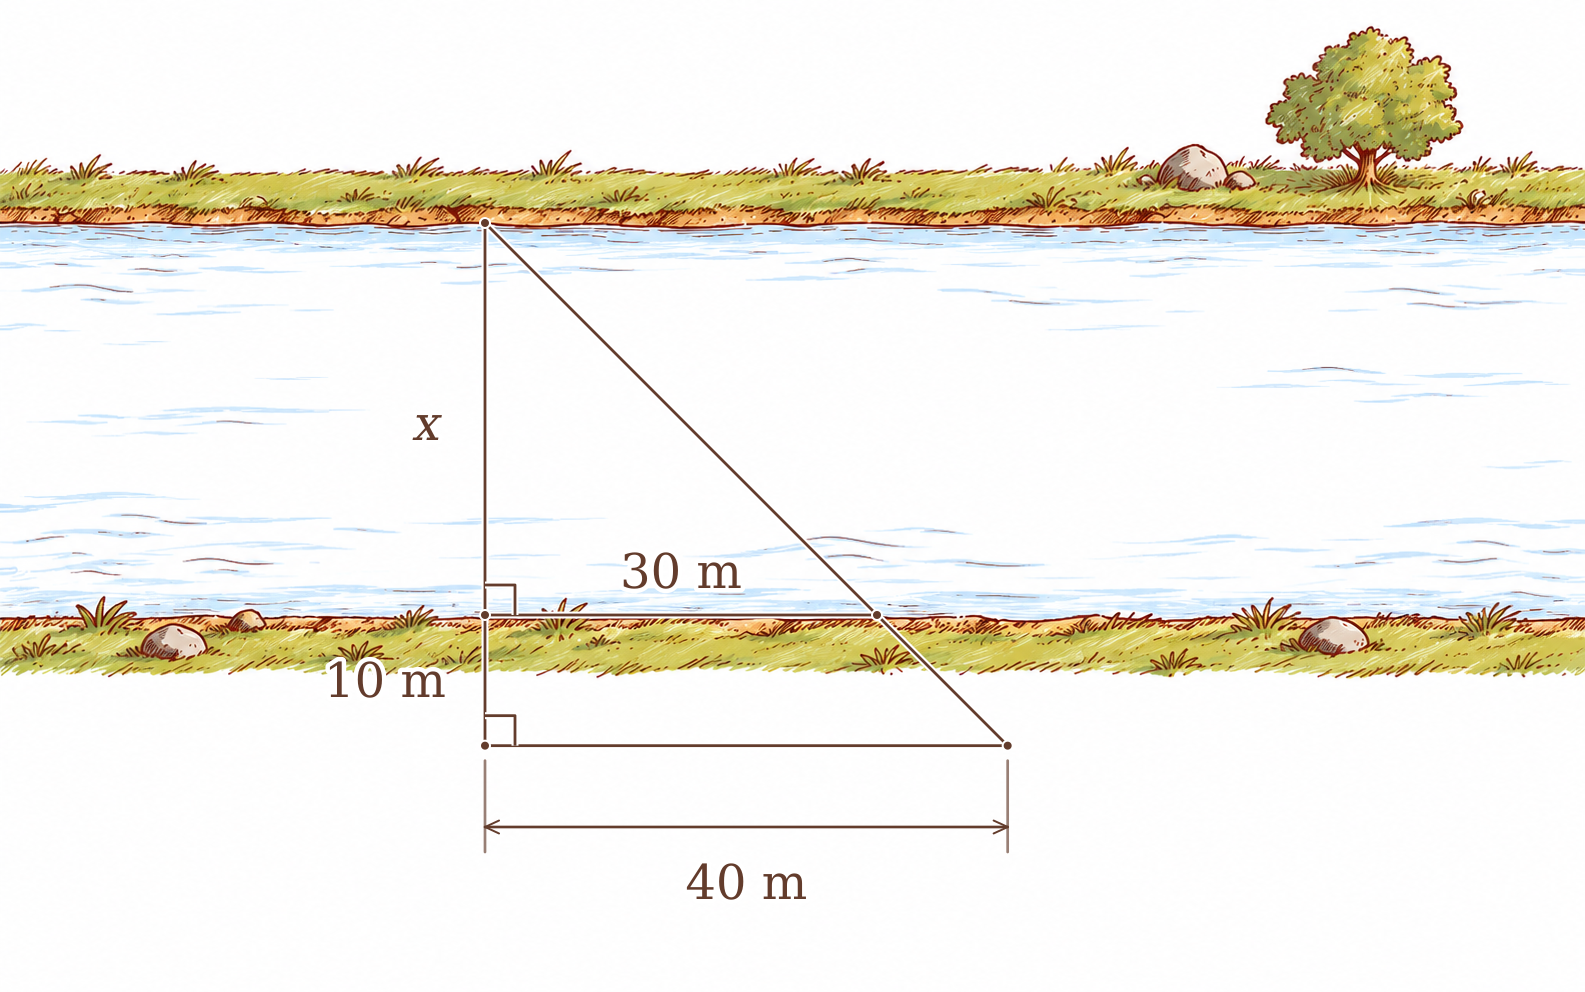
\includegraphics[width=.70\linewidth,height=55mm,keepaspectratio]{images/lota28_t3_armaeling.png}\end{mynd}
Litli þríhyrningurinn hefur hæð \(x\) og grunnlínu \(30\metri\). Sá stóri hefur hæð \(x+10\) og grunnlínu \(40\metri\). Þeir hafa sameiginlegt efsta horn og rétt horn við grunnlínurnar.
\[\begin{aligned}
&\frac{x}{x+10}=\frac{30}{40}\\[5pt]&40x=30(x+10)\\[5pt]&10x=300\\[5pt]&x=30\metri.
\end{aligned}\]
Prófun: \(\frac{30}{40}=\frac{30}{30+10}\).
\end{daemi}

\begin{mundu}\textbf{ATH.:} Ef nauðsynlega lengd vantar er ekki hægt að finna ákveðið tölusvar. Kallaðu lengdina \(b\) og skrifaðu sambandið með \(b\), eða aflaðu mælingarinnar. Ekki lesa ómerkta lengd af skissu.\end{mundu}

\timi{4}{MÆLIKVARÐI}
\markmid{Að finna og nota mælikvarða, samræma einingar og reikna raunverulegar lengdir og flatarmál út frá mynd.}
\kafli{Mynd á móti raunveruleika}
\hugtak{maelikvardi}{Mælikvarði} er hlutfall lengdar á mynd og samsvarandi lengdar í raunveruleikanum. Báðar lengdir verða að vera í sömu einingu áður en hlutfallið er stytt.
\begin{regla}\textbf{FLÝTILEIÐ:} Við notum röðina \textbf{mynd : raun}.
\[\begin{aligned}
&a:b\\[5pt]&\text{Raunlengd}=\text{myndlengd}\cdot\frac ba\\[5pt]&\text{myndlengd}=\text{Raunlengd}\cdot\frac ab.
\end{aligned}\]
\(1:n\) með \(n>1\) er minnkun; \(n:1\) með \(n>1\) er stækkun.\end{regla}
\begin{daemi}{Finna mælikvarða líkans}
Turn er \(72\metri\) á hæð og líkan af honum \(4{,}5\cm\).
\begin{mynd}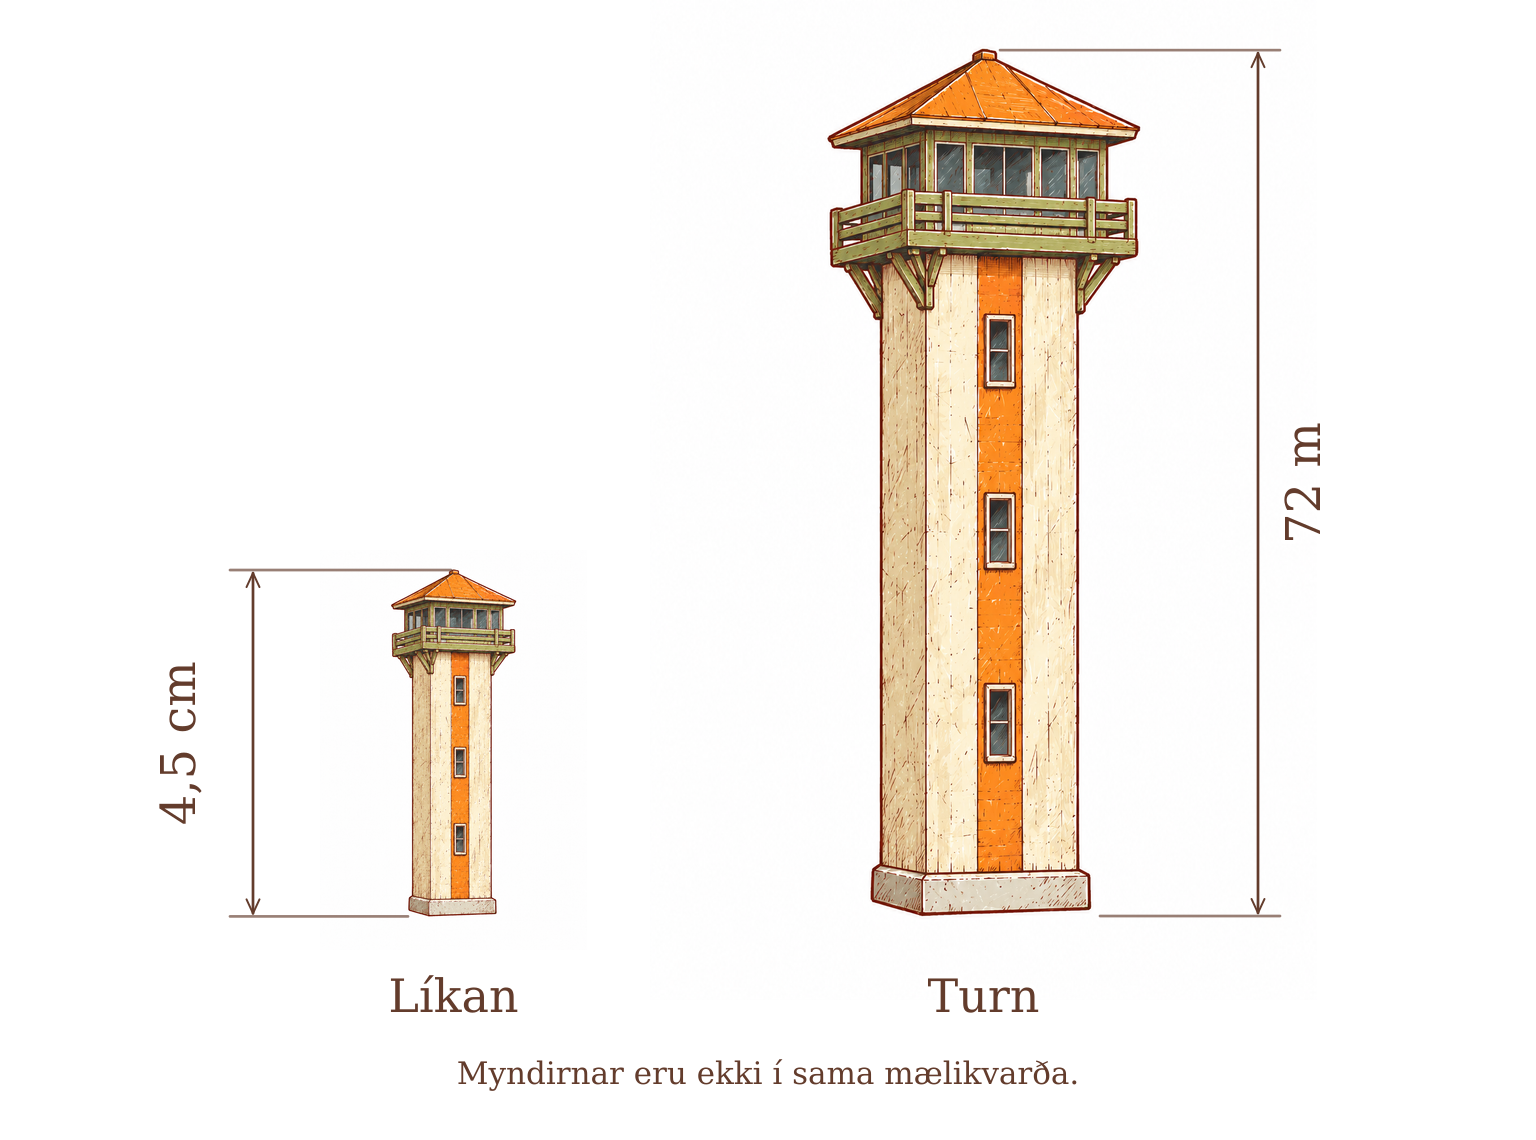
\includegraphics[width=.70\linewidth,height=55mm,keepaspectratio]{images/lota28_t4_turn_og_likan.png}\end{mynd}
\[\begin{aligned}
&72\metri=7200\cm\\[5pt]&4{,}5:7200=1:1600.
\end{aligned}\]
Líkanið er í mælikvarðanum \(\bla{1:1600}\). Einn sentímetri á líkaninu táknar \(1600\cm=16\metri\).
\end{daemi}
\begin{daemi}[lotaCyan]{Óvenjulegir mælikvarðar}
\begin{tabularx}{\linewidth}{@{}l l X@{}}
\toprule
\textbf{Gefið}&\textbf{Stytt}&\textbf{Túlkun}\\\midrule
\(3:750\,000\)&\(1:250\,000\)&Minnkun; \(1\cm\) táknar \(2{,}5\,\text{km}\).\\
\(180:12\)&\(15:1\)&Stækkun; myndlengd er 15 sinnum raunlengd.\\\bottomrule
\end{tabularx}
Við stækkun í \(15:1\) er \(6\cm\) myndlengd aðeins \(\frac{6}{15}=0{,}4\cm\) í raun.
\end{daemi}
\kafli{Lengdir á landakorti}
\begin{daemi}[lotaMagenta]{Nota kvarða á landakorti}
Á korti í mælikvarðanum \(1:350\,000\) mælist leið \(7{,}2\cm\). Raunlengdin er

\[\begin{aligned}
&7{,}2\cdot350\,000=2\,520\,000\cm=25{,}2\,\text{km}.
\end{aligned}\]
\end{daemi}

\framhald{MÆLINGAR OG FLATARMÁL Á KORTI}
\kafli{Mældu með viðmiði}
Ef þekkt raunlengd er merkt á mynd geturðu notað hana til að finna mælikvarðann. Veldu skýra endapunkta. Mældu allar lengdir á sömu útgáfu myndarinnar.
\begin{daemi}{Húsgafl með þekktri hæð}
Hæð gafls er \(6\metri\) í raun. Á útprentun mælist hún \(4\cm\), en breiddin \(6\cm\). Þá er
\[\begin{aligned}
&4:600=1:150\\[5pt]&\text{Breidd}=6\cdot150\\[5pt]&=900\cm\\[5pt]&=9\metri.
\end{aligned}\]
Sama svar fæst beint úr hlutfalli: \(\frac{6}{4}\cdot6=9\metri\).
\begin{mynd}
\begin{tikzpicture}[x=1cm,y=1cm]
% Raunveruleg prentstærð varðveitt: myndin er 6 cm x 4 cm.
\draw[fill=lotaYellow!20] (0,0)--(6,0)--(6,2.4)--(3,4)--(0,2.4)--cycle;
\draw[dashed,lotaBlue](3,0)--(3,4);
\draw[hjalparlina](6,0)--(6.95,0) (3,4)--(6.95,4);
\draw[mal](6.75,0)--node[maltexti,right=5pt,align=left]{$4\cm$\\á mynd}(6.75,4);
\draw[hjalparlina](0,0)--(0,-.9) (6,0)--(6,-.9);
\draw[mal](0,-.7)--node[maltexti,below=4pt]{$6\cm$ á mynd}(6,-.7);
\end{tikzpicture}
\end{mynd}
Myndin er teiknuð \(6\cm\) breið og \(4\cm\) há í PDF-skjalinu. Til að staðfesta þetta með reglustiku þarf að prenta í \textbf{100\% / raunverulegri stærð}.
\end{daemi}
\begin{mundu}\textbf{MUNDU:} Stækkun á skjá eða „laga að blaðsíðu“ við prentun breytir mælikvarðanum sem þú mælir. Hlutfall tveggja lengda helst þó óbreytt ef myndin er stækkuð eða minnkuð jafnt í allar áttir.\end{mundu}
\kafli{Flatarmál fær tvo lengdarstuðla}
\begin{daemi}[lotaMagenta]{Frá fersentímetrum yfir í ferkílómetra}
Á korti táknar \(1\cm\) lengdina \(3\,\text{km}\). Einn \(1\cm\times1\cm\) reitur táknar því \(3\,\text{km}\times3\,\text{km}=9\,\text{km}^2\).
\[\begin{aligned}
&\text{Flatarmál á korti}=120\,\text{cm}^2\\[5pt]&\text{Raunverulegt flatarmál}=120\cdot9\\[5pt]&=1080\,\text{km}^2.
\end{aligned}\]
Lengdarkvarðinn er \(1:300\,000\). Nota má hann í öðru veldi, en þá þarf einnig að breyta \(\text{cm}^2\) í \(\text{km}^2\). Reitaleiðin hér að ofan heldur einingunum sýnilegum.
\end{daemi}
\timi{5}{MÆLIKVARÐAR OG VINNUTEIKNINGAR}
\markmid{Að lesa reitasnið, skipuleggja efnisnotkun, gera efnislista og teikna samræmda grunnmynd, mynd framan frá og mynd frá hlið.}
\kafli{Reitur getur táknað mismunandi lengdir}
Á \hugtak{vinnuteikning}{vinnuteikningu} þurfa mál, einingar og mælikvarði að vera skýr. Á reitasniði telurðu fyrst reitina og margfaldar síðan með lengdinni sem einn reitur táknar. Teldu \emph{bilin milli lína}, ekki línurnar.
\begin{daemi}{Snið á samanbrotnu efni}
Hálft snið af hlíf er \(7\) reitir á lengd og mest \(3\) reitir á breidd. Beina brúnin liggur við brot efnisins. Þegar það er opnað verður hlífin mest \(6\) reitir á breidd.

\begin{mynd}
\begin{tikzpicture}[scale=.55]
\fill[lotaCyan!25](0,0)--(3,0)--(3,5)--(2,7)--(0,7)--cycle;
\draw[step=1,gray!50,thin] (0,0)grid(4,8);
\draw[thick](0,0)--(3,0)--(3,5)--(2,7)--(0,7)--cycle;
\draw[lotaBlue,very thick](0,0)--(0,7);
\node[rotate=90,anchor=south,inner sep=3pt]at(-.55,3.5){brot efnisins};
\draw[hjalparlina](3,0)--(5.1,0) (2,7)--(5.1,7);
\draw[mal](4.85,0)--node[maltexti,right=5pt]{7 reitir}(4.85,7);
\draw[hjalparlina](0,0)--(0,-1.3) (3,0)--(3,-1.3);
\draw[mal](0,-1.05)--node[maltexti,below=4pt]{3 reitir}(3,-1.05);
\end{tikzpicture}
\end{mynd}Ef reitur táknar \(8\cm\) verður lengdin \(7\cdot8=56\cm\) og mesta breiddin \(2\cdot3\cdot8=48\cm\).

\end{daemi}
\kafli{Hve marga metra af efni þarf?}
Raðaðu sniðunum á efnið og athugaðu hvort þau rúmast á breidd þess. Uppstillingin ræður hversu langa efnisræmu þarf. Taktu tillit til saumfara, afskurðar og mynsturstefnu; flatarmálið eitt segir ekki hvort sniðin passa.

\framhald{EFNISLISTI ÚR VINNUTEIKNINGU}
\kafli{Teldu hluti áður en þú leggur saman lengdir}
\hugtak{efnislisti}{Efnislisti} sýnir tegund efnis, fjölda stykkja, lengd hvers stykkis og heildarlengd. Sami hlutur getur sést á fleiri en einni mynd; teldu hann aðeins einu sinni.
\begin{daemi}{Tveir samliggjandi kassar}
Í þessu dæmi eru kassarnir samtals \(1{,}8\metri\) breiðir og \(0{,}6\metri\) djúpir. Þeir hafa sameiginlegan millivegg. Bæði á framhlið og bakhlið eru fjórar samfelldar raðir af \(1{,}8\metri\) borðum. Á hvorri endahlið og á milliveggnum eru fjórar raðir af \(0{,}6\metri\) borðum. Sex stólpar eru hver \(1{,}1\metri\).
\begin{mynd}
\begin{tikzpicture}[x=3.5cm,y=3.5cm]
\draw[fill=lotaYellow!18](0,0)rectangle(1.8,.6);\draw(.9,0)--(.9,.6);
\foreach \x in {0,.9,1.8}{\foreach \y in {0,.6}{\fill[lotaStep](\x-.035,\y-.035)rectangle(\x+.035,\y+.035);}}
\draw[hjalparlina](0,0)--(0,-.3) (1.8,0)--(1.8,-.3) (1.8,0)--(2.1,0) (1.8,.6)--(2.1,.6);
\draw[mal](0,-.23)--node[maltexti,below=4pt]{$1{,}8\metri$}(1.8,-.23);
\draw[mal](2.04,0)--node[maltexti,right=5pt]{$0{,}6\metri$}(2.04,.6);
\node[anchor=south] at (.9,.85){Grunnmynd};
\end{tikzpicture}
\end{mynd}
\begin{tabularx}{\linewidth}{@{}X r r r@{}}
\toprule
\textbf{Efni og staður}&\textbf{Fjöldi}&\textbf{Lengd}&\textbf{Samtals}\\\midrule
Borð, framhlið og bakhlið&8&\(1{,}8\metri\)&\(14{,}4\metri\)\\
Borð, endar og milliveggur&12&\(0{,}6\metri\)&\(7{,}2\metri\)\\
Stólpar&6&\(1{,}1\metri\)&\(6{,}6\metri\)\\\bottomrule
\end{tabularx}
Heildarlengd borða er \(14{,}4+7{,}2=\bla{21{,}6\metri}\). Stólpaefnið er talið sér: \(\bla{6{,}6\metri}\).
\end{daemi}
\kafli{Lesa mál og efnismerkingar}
Merkingar á borð við \(1\times6\) tommur og \(2\times2\) tommur vísa til nafnmáls þversniðs timburs, ekki lengdar hvers stykkis. Skráðu efnisgerðirnar í aðskildum línum. Ein tomma er \(2{,}54\cm\), en nafnmál og raunmál unnins timburs geta verið ólík.

Ef stólpi nær bæði upp úr og niður í jörð þarf að leggja saman lengdir beggja hluta. Til dæmis gefa \(0{,}7\metri\) ofanjarðar og \(0{,}4\metri\) neðanjarðar heildarlengdina \(1{,}1\metri\).
\begin{mundu}\textbf{MUNDU:} Efnislistinn byggist á málunum og fjölda stykkja í dæminu. Við smíði þarf einnig að huga að samskeytum, þykkt efnis, afskurði og þeim lengdum sem efnið fæst í. Ekki mæla skálengdir af þrívíddarskissu eins og þær séu í sama mælikvarða og grunnmynd.\end{mundu}

\framhald{GRUNNMYND, MYND FRAMAN FRÁ OG MYND FRÁ HLIÐ}
\kafli{Þrjár myndir af sama hlut}
\hugtak{grunnmynd}{Grunnmynd} sýnir hlut ofan frá: lengd og breidd. \hugtak{framsyn}{Mynd framan frá} sýnir breidd og hæð þegar horft er beint framan á hlutinn. \hugtak{hlidarsyn}{Mynd frá hlið} sýnir lengd og hæð. Sama mál þarf að passa á öllum myndunum þar sem það kemur fyrir.
\begin{daemi}{Lítið geymsluhús í mælikvarðanum 1:20}
Við \emph{veljum} eftirfarandi mál fyrir reiknidæmið: lengd \(120\cm\), breidd \(90\cm\), vegghæð \(80\cm\) og hæð í mæni \(110\cm\). Op að framan er \(40\cm\) breitt og \(60\cm\) hátt.
\[\begin{array}{c|rrrrrr}
\text{Raunlengd (cm)}&120&90&80&110&40&60\\
\text{Á teikningu (cm)}&6&4{,}5&4&5{,}5&2&3
\end{array}\]
Tölurnar við teikninguna sýna \emph{raunmálin}, þótt lengdirnar á blaðinu séu styttri.
\end{daemi}
\begin{mynd}
\begin{tikzpicture}[x=1cm,y=1cm,font=\small]
% Sýnirnar haldast allar í 1:20. Aðeins bil og málsetningar eru færð.
\begin{scope}
\draw[fill=lotaCyan!12](0,0)rectangle(4.5,6);
\draw[hjalparlina](0,0)--(-.8,0) (0,6)--(-.8,6) (0,0)--(0,-.8) (4.5,0)--(4.5,-.8);
\draw[mal](-.6,0)--node[maltexti,left=4pt]{120 cm}(-.6,6);
\draw[mal](0,-.6)--node[maltexti,below=4pt]{90 cm}(4.5,-.6);
\node[anchor=south,font=\normalsize\bfseries] at (2.25,6.55){GRUNNMYND};
\end{scope}
\begin{scope}[xshift=6.6cm,yshift=3cm]
\draw[fill=lotaYellow!20](0,0)--(4.5,0)--(4.5,4)--(2.25,5.5)--(0,4)--cycle;
\draw[fill=white](1.25,0)rectangle(3.25,3);
\draw[hjalparlina](4.5,0)--(5.35,0) (2.25,5.5)--(5.35,5.5);
\draw[mal](5.15,0)--node[maltexti,right=4pt]{110 cm}(5.15,5.5);
\draw[hjalparlina](0,0)--(0,-.8) (4.5,0)--(4.5,-.8);
\draw[mal](0,-.6)--node[maltexti,below=4pt]{90 cm}(4.5,-.6);
\node[anchor=south,font=\normalsize\bfseries] at (2.25,6.05){MYND FRAMAN FRÁ};
\node[align=center] at (2.25,1.5){40 $\times$ 60\\cm};
\end{scope}
\begin{scope}[xshift=5.5cm,yshift=-5cm]
\draw[fill=lotaGreen!10](0,0)rectangle(6,5.5);\draw(0,4)--(6,4);
\draw[hjalparlina](0,0)--(0,-.8) (6,0)--(6,-.8) (6,0)--(6.85,0) (6,4)--(6.85,4);
\draw[mal](0,-.6)--node[maltexti,below=4pt]{120 cm}(6,-.6);
\draw[mal](6.65,0)--node[maltexti,right=4pt]{80 cm}(6.65,4);
\node[anchor=south,font=\normalsize\bfseries] at (3,5.95){MYND FRÁ HLIÐ};
\end{scope}
\end{tikzpicture}
\end{mynd}
Myndirnar eru í kvarðanum \(1:20\) við prentun í 100\%. Þær sýna ytri mál; veggþykkt er ekki útfærð. Þegar verkefni gefur aðeins hæð dýrs eða notkun húss þarftu að velja önnur mál og taka skýrt fram hvaða mál þú valdir.

\framhald{GRUNNTEIKNING OG GÓLFFLÖTUR}
\kafli{Athugaðu einingar og línur sem sýna mál}
Byggingateikningar eru oft málsettar í millímetrum. Talan \(3200\) getur þá táknað \(3200\,\text{mm}=3{,}2\metri\). Athugaðu einingaskýringu; ef hún vantar skaltu rökstyðja túlkun út frá raunhæfri stærð herbergisins og búnaðarins.

Notaðu innanmál herbergisins til að finna flatarmál gólfsins. Áætlaðu með einföldum formum hve stóran flöt búnaðurinn þekur og leggðu flatarmál þeirra saman án skörunar. Til að fá prósentu deilirðu flatarmáli undir búnaðinum með flatarmáli alls gólfsins og margfaldar með \(100\%\).

\begin{mundu}\textbf{ATH.:} Skoðaðu hvort málin eiga við fjarlægð milli innri veggflata eða ytri brúna. Flatarmál veggjanna á ekki að telja með gólffleti herbergisins. Boginn við hurð sýnir opnun hennar; hann er ekki fastur búnaður sem þekur gólfið.\end{mundu}

\framhald{FRÁ TVÍVÍDD AÐ ÞRÍVÍDD}
\kafli{Þrjár stefnur á punktablaði}
Á \hugtak{thrividd}{þrívíddarteikningu} sjást lengd, breidd og hæð. Á jafnhalla punktaneti eru tvær stefnur skáhallar og sú þriðja lóðrétt. Teldu jafn löng skref eftir hverri stefnu; mældu ekki lárétta breidd skáhalla hlutarins á blaðinu sem raunlengd.
\begin{daemi}{Kassi úr einingum}
Kassi er \(80\cm\) langur, \(40\cm\) djúpur og \(60\cm\) hár. Eitt bil milli punkta táknar \(20\cm\). Þá þarf 4 bil í lengd, 2 í dýpt og 3 í hæð.
\begin{mynd}
\begin{tikzpicture}[x={(.84cm,.48cm)},y={(-.84cm,.48cm)},z={(0cm,.96cm)}]
\foreach \i in {-1,...,5}{\foreach \j in {-1,...,3}{\fill[gray!55](\i,\j,0)circle(.7pt);}}
\fill[lotaCyan!25](0,0,0)--(4,0,0)--(4,0,3)--(0,0,3)--cycle;
\fill[lotaGreen!20](0,0,0)--(0,2,0)--(0,2,3)--(0,0,3)--cycle;
\fill[lotaYellow!35](0,0,3)--(4,0,3)--(4,2,3)--(0,2,3)--cycle;
\draw(0,0,0)--(4,0,0)--(4,0,3)--(4,2,3)--(0,2,3)--(0,2,0)--cycle;
\draw(0,0,0)--(0,0,3)--(4,0,3) (0,0,3)--(0,2,3);
\foreach \i in {1,2,3}{\draw[gray!60,thin](\i,0,0)--(\i,0,3)--(\i,2,3);}
\foreach \j in {1,2}{\draw[gray!60,thin](0,0,\j)--(4,0,\j) (0,0,\j)--(0,2,\j);}
\draw[gray!60,thin](0,1,0)--(0,1,3)--(4,1,3);
\draw[hjalparlina](0,0,0)--(0,-.75,0) (4,0,0)--(4,-.75,0);
\draw[mal](0,-.55,0)--node[midway,sloped,below=4pt,maltexti]{80 cm}(4,-.55,0);
\draw[hjalparlina](0,0,0)--(-.75,0,0) (0,2,0)--(-.75,2,0);
\draw[mal](-.55,0,0)--node[midway,sloped,below=4pt,maltexti]{40 cm}(-.55,2,0);
\draw[hjalparlina](4,0,0)--(4.85,0,0) (4,0,3)--(4.85,0,3);
\draw[mal](4.65,0,0)--node[midway,right=5pt,maltexti]{60 cm}(4.65,0,3);
\end{tikzpicture}
\end{mynd}
Grunnmynd kassans er rétthyrningur, 4 bil á móti 2. Mynd framan frá er 4 bil á móti 3 og mynd frá hlið 2 bil á móti 3. Þrívíddarmyndin sameinar þessar upplýsingar.
\end{daemi}
\kafli{Skipuleg vinnuröð}
\begin{enumerate}
\item Skráðu raunmálin og hvað er gefið eða valið.
\item Veldu mælikvarða þannig að myndin rúmist á blaðinu og reiknaðu lengdirnar á teikningunni.
\item Teiknaðu grunnmynd fyrst og sýndu innbyrðis staðsetningu hlutanna.
\item Teiknaðu mynd framan frá og mynd frá hlið þannig að samsvarandi mál passi saman.
\item Bættu við línum sem sýna mál, raunmálum, einingum og mælikvarða.
\item Ef þrívíddarmynd fylgir skaltu yfirfæra sömu mál á þrjár stefnur punktanetsins.
\end{enumerate}
\begin{mundu}\textbf{MUNDU:} Þrívíddarmynd hjálpar þér að sjá hlutinn fyrir þér. Grunnmynd, mynd framan frá og mynd frá hlið með skráðum málum sýna nákvæmar stærðir. Báðar gerðir geta verið gagnlegar í sama verkefni.\end{mundu}


\timi{6}{FLATARMÁL, UMMÁL OG RÚMMÁL}
\markmid{Að velja rétta stærð og einingu, finna hæð þríhyrnings og reikna rúmmál einfaldra og samsettra forma.}
\kafli{Jaðar, flötur eða rými?}
\hugtak{ummal}{Ummál} \(U\) er lengd jaðars og er til dæmis mælt í cm. \hugtak{flatarmal}{Flatarmál} \(F\) segir hversu stór flötur er og er til dæmis mælt í cm\(^2\). \hugtak{rummal}{Rúmmál} \(R\) mælir rými og er til dæmis mælt í cm\(^3\).
\begin{regla}\textbf{FLÝTILEIÐ:}
\begin{tabularx}{\linewidth}{@{}X l l@{}}
\textbf{Form}&\textbf{Ummál}&\textbf{Flatarmál}\\\midrule
Ferningur, hlið \(h\)&\(U=4h\)&\(F=h^2\)\\
Rétthyrningur, hliðar \(l,b\)&\(U=2(l+b)\)&\(F=lb\)\\
Þríhyrningur, hliðar \(a,b,c\)&\(U=a+b+c\)&\(F=\frac{l\cdot h}{2}\)\\
Hringur, radíus \(r\)&\(U=2\pi r\)&\(F=\pi r^2\)
\end{tabularx}
Í þríhyrningsformúlunni er \(h\) hornrétt á grunnlínuna \(l\). Í ferningsformúlunum táknar \(h\) hliðarlengd ferningsins.\end{regla}
\begin{daemi}{Sömu hliðarlengdir, ólíkar stærðir}
Rétthyrningur með hliðar \(7\cm\) og \(3{,}5\cm\) hefur

\[\begin{aligned}
&U=2(7+3{,}5)=21\cm\\[5pt]&F=7\cdot3{,}5=24{,}5\,\text{cm}^2.
\end{aligned}\]
\end{daemi}
\kafli{Hæð má liggja utan þríhyrnings}
\begin{mynd}
\begin{tikzpicture}[scale=.62]
\draw[fill=lotaCyan!15](0,0)--(6,0)--(2,4)--cycle;
\draw[dashed](2,0)--node[midway,maltexti,right=5pt]{$4$}(2,4);
\draw(2,.35)--(2.35,.35)--(2.35,0);\node[maltexti,below=5pt]at(3,0){$6$};
\begin{scope}[xshift=10cm]
\draw[fill=lotaGreen!15](0,0)--(4,0)--(6,3)--cycle;
\draw[dashed](4,0)--(6,0)--node[midway,maltexti,right=5pt]{$3$}(6,3);
\draw(5.65,0)--(5.65,.35)--(6,.35);\node[maltexti,below=5pt]at(2,0){$4$};
\end{scope}
\end{tikzpicture}
\end{mynd}
\begin{daemi}[lotaCyan]{Veldu grunnlínu og tilheyrandi hæð}
Vinstra megin er

\[\begin{aligned}
&F=\frac{6\cdot4}{2}=12
\end{aligned}\]
flatareiningar. Hægra megin er

\[\begin{aligned}
&F=\frac{4\cdot3}{2}=6
\end{aligned}\]
flatareiningar. Hæðin er alltaf hornrétt fjarlægð frá hornpunktinum gegnt grunnlínunni að línunni sem hún liggur á, jafnvel þegar hún liggur utan þríhyrningsins.

\end{daemi}

\framhald{HRINGUR, KASSI OG HLASS}
\begin{daemi}{Stærra ummál tryggir ekki stærra flatarmál}
Berum saman ferning með hlið \(7\metri\) og hring með \hugtak{radius}{radíus} \(4\metri\).
\[\begin{array}{c|cc}
&\text{Ferningur}&\text{Hringur}\\\hline
U&28\metri&8\pi\metri\approx25{,}13\metri\\
F&49\,\text{m}^2&16\pi\,\text{m}^2\approx50{,}27\,\text{m}^2
\end{array}\]
Ferningurinn hefur stærra ummál en hringurinn stærra flatarmál. Á mynd skaltu athuga hvort merkt strik liggur frá miðju að jaðri (radíus) eða þvert yfir hringinn gegnum miðju (þvermál).
\end{daemi}
\kafli{Rúmmál sem lög af einingateningum}
Í kassa með rétthyrnda fleti eru \(l\cdot b\) einingaferningar í botninum. Hæðin segir hve mörg lög af einingateningum komast ofan á hann. Því er \(R=lbh\).
\begin{regla}\textbf{FLÝTILEIÐ:} Fyrir \hugtak{rettstrendingur}{réttstrending} er
\[\begin{aligned}
&R=G\cdot h
\end{aligned}\]
þar sem \(G\) er flatarmál grunnflatar og \(h\) hornrétt hæð. Fyrir rétthyrndan kassa er \(G=l\cdot b\), svo \(R=lbh\).\end{regla}
\begin{daemi}[lotaCyan]{Þegar flatarmál grunnflatar er þekkt}
Réttstrendingur hefur grunnflöt með flatarmálinu \(G=32{,}5\,\text{m}^2\) og hæðina \(h=1{,}2\metri\). Þá er

\[\begin{aligned}
&R=32{,}5\cdot1{,}2=39\,\text{m}^3.
\end{aligned}\]
Við þurfum ekki hliðarlengdir grunnflatarins ef flatarmál hans er þegar þekkt.

\end{daemi}
\begin{daemi}[lotaMagenta]{Massi reiknaður út frá rúmmáli}
Farmrými vagns er \(5\metri\) langt, \(2{,}2\metri\) breitt og fyllt í \(0{,}6\metri\) hæð. Gerum ráð fyrir kassalaga farmrými og að hver rúmmetri af efninu vegi \(1{,}4\) tonn.
\begin{mynd}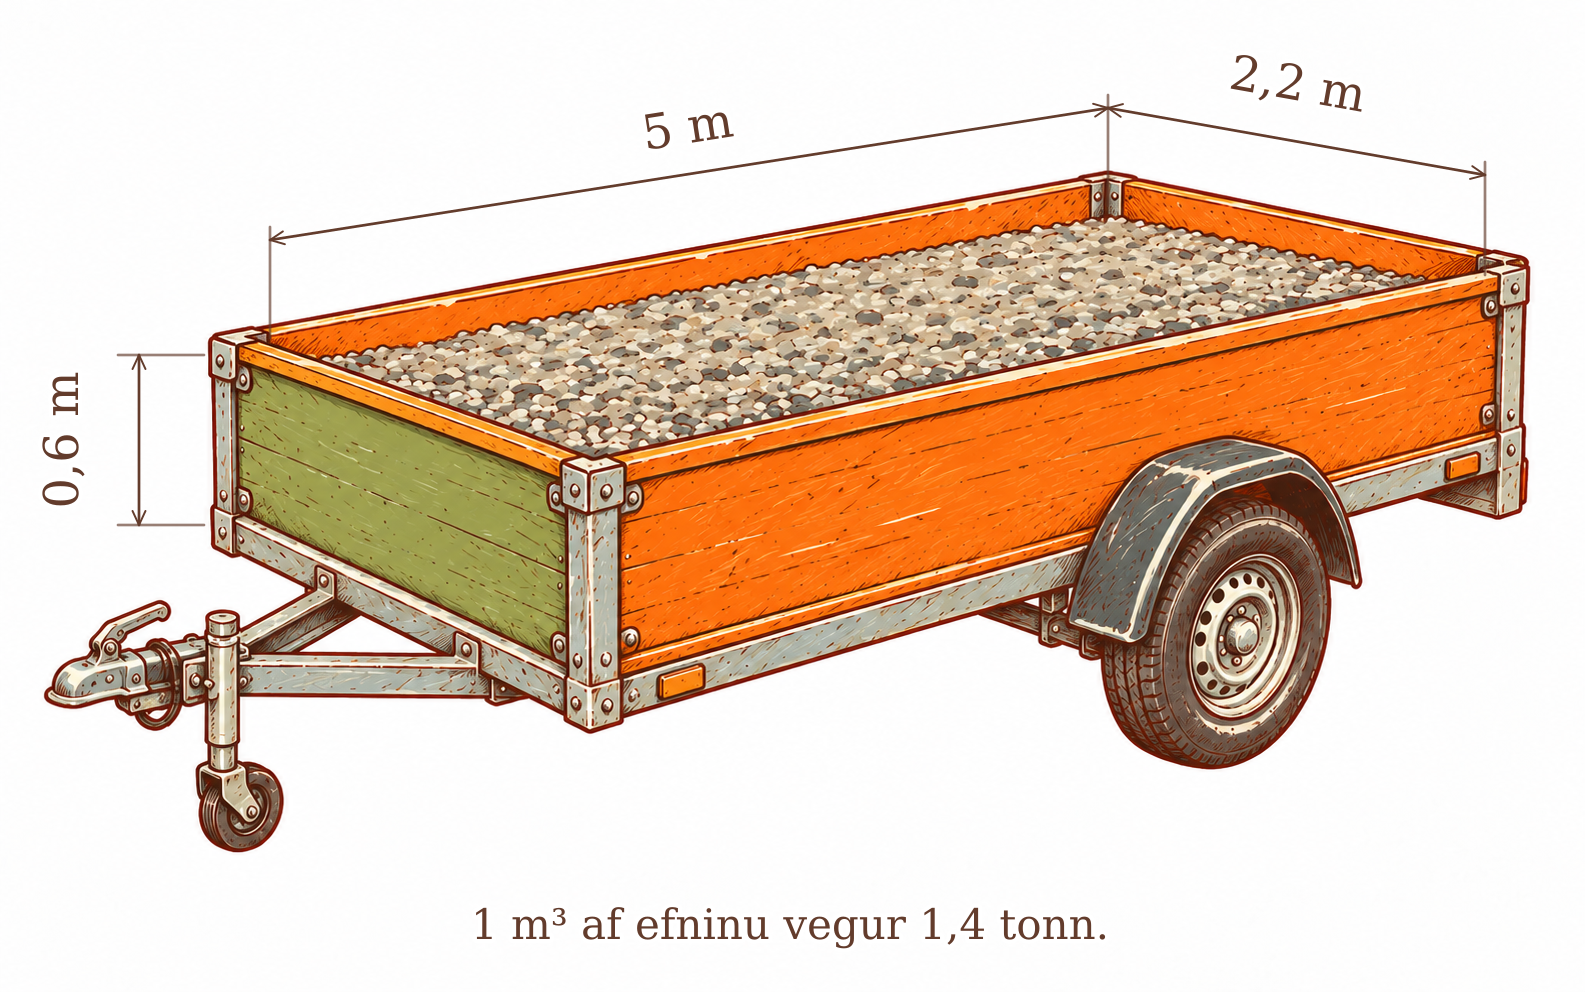
\includegraphics[width=.70\linewidth,height=55mm,keepaspectratio]{images/lota28_t6_malarvagn.png}\end{mynd}
\[\begin{aligned}
&R=5\cdot2{,}2\cdot0{,}6\\[5pt]&R=6{,}6\,\text{m}^3\\[5pt]&m=6{,}6\cdot1{,}4=9{,}24\text{ tonn}.
\end{aligned}\]
Hér táknar \(m\) massa efnisins í tonnum. Massi vagnsins sjálfs er ekki innifalinn.
\end{daemi}

\framhald{ÓLÍK MÁL OG SAMSETT FORM}
\kafli{Mörg form geta haft sama rúmmál}
\begin{daemi}{Finndu mál þegar rúmmálið er þekkt}
Kassi hefur rúmmálið \(72\,\text{dm}^3\), lengdina \(3\,\text{dm}\) og breiddina \(4\,\text{dm}\). Hæðin fæst með því að deila rúmmálinu með flatarmáli botnsins:

\[\begin{aligned}
&h=\frac{72}{3\cdot4}=6\,\text{dm}.
\end{aligned}\]
Ef aðeins rúmmálið er gefið eru margar mögulegar samsetningar lengdar, breiddar og hæðar.

\end{daemi}
\kafli{L-laga kubbur: heill kassi mínus horn}
\begin{mynd}
\begin{tikzpicture}[scale=.38]
\fill[lotaCyan!20](0,0)--(9,0)--(9,4)--(15,4)--(15,10)--(0,10)--cycle;
\draw[thick](0,0)--(9,0)--(9,4)--(15,4)--(15,10)--(0,10)--cycle;
\draw[dashed,lotaMagenta](9,0)--(15,0)--(15,4);
\draw[mal](0,-2)--node[maltexti,below=4pt]{$15\cm$}(15,-2);
\draw[mal](-2,0)--node[maltexti,left=4pt]{$10\cm$}(-2,10);
\draw[mal](9,2)--node[maltexti,above=4pt]{$6\cm$}(15,2);
\draw[mal](17,0)--node[maltexti,right=4pt]{$4\cm$}(17,4);
\node[anchor=south] at (7.5,11.2){Grunnmynd ofan frá};
\node[anchor=north] at (7.5,-4.5){Hæð kubbsins er $3\cm$.};
\end{tikzpicture}
\end{mynd}
\begin{daemi}[lotaMagenta]{Tvær leiðir að rúmmáli L-laga kubbs}
Úr kassa sem er \(15\cm\) langur, \(10\cm\) breiður og \(3\cm\) hár er tekið rétthyrnt horn, \(6\cm\) á móti \(4\cm\), alla leið niður.

\textbf{Heill kassi mínus hornið:}

\[\begin{aligned}
&R=15\cdot10\cdot3-6\cdot4\cdot3\\[5pt]&R=450-72=378\,\text{cm}^3.
\end{aligned}\]
\textbf{Tveir kassar lagðir saman:} Skiptum L-laga grunnfletinum í rétthyrninga með mál \(9\cm\times10\cm\) og \(6\cm\times6\cm\). Báðir kassar eru \(3\cm\) háir.

\[\begin{aligned}
&R=9\cdot10\cdot3+6\cdot6\cdot3\\[5pt]&R=270+108=378\,\text{cm}^3.
\end{aligned}\]
\end{daemi}
\begin{mundu}\textbf{MUNDU:} Þegar hluti er tekinn úr kassa dregurðu rúmmál þess hluta frá rúmmáli alls kassans. Ef þú leggur saman rúmmál minni kassa mega þeir ekki skarast.\end{mundu}
\timi{7}{RÚMMÁL OG EININGABREYTINGAR}
\markmid{Að breyta milli rúmeininga og lítraeininga og tengja rúmmál vatns við massa samkvæmt gefinni forsendu.}
\kafli{Hvers vegna margföldum við með þúsund?}
Einn desímetri er tíu sentímetrar. Teningur með brún \(1\,\text{dm}\) hefur því 10 sentímetra í hverja af þremur áttum:
\[\begin{aligned}
&1\,\text{dm}^3=(10\cm)^3\\[5pt]&=10\cdot10\cdot10\,\text{cm}^3\\[5pt]&=1000\,\text{cm}^3.
\end{aligned}\]
\begin{mynd}
\begin{tikzpicture}[x={(.32cm,0cm)},y={(.14cm,.11cm)},z={(0cm,.32cm)}]
\fill[lotaCyan!15](0,0,0)--(10,0,0)--(10,0,10)--(0,0,10)--cycle;
\fill[lotaYellow!25](0,0,10)--(10,0,10)--(10,10,10)--(0,10,10)--cycle;
\fill[lotaGreen!18](10,0,0)--(10,10,0)--(10,10,10)--(10,0,10)--cycle;
\foreach \i in {0,...,10}{\draw[gray!65,thin](\i,0,0)--(\i,0,10)--(\i,10,10);
\draw[gray!65,thin](0,0,\i)--(10,0,\i)--(10,10,\i);
\draw[gray!65,thin](0,\i,10)--(10,\i,10)--(10,\i,0);}
\draw[hjalparlina](0,0,0)--(0,0,-2.4) (10,0,0)--(10,0,-2.4);
\draw[mal](0,0,-1.9)--node[midway,maltexti,below=4pt]{10 cm}(10,0,-1.9);
\draw[hjalparlina](10,0,0)--(12.8,0,0) (10,10,0)--(12.8,10,0);
\draw[mal](12.3,0,0)--node[midway,sloped,below=5pt,maltexti]{10 cm}(12.3,10,0);
\draw[hjalparlina](10,10,0)--(13.3,10,0) (10,10,10)--(13.3,10,10);
\draw[mal](12.8,10,0)--node[midway,maltexti,right=5pt]{10 cm}(12.8,10,10);
\end{tikzpicture}
\end{mynd}
\begin{regla}\textbf{FLÝTILEIÐ:} Í hverju skrefi til hægri margföldum við með þúsund:
\[\begin{aligned}
&\text{m}^3 \xrightarrow{ \times1000 } \text{dm}^3
 \xrightarrow{ \times1000 } \text{cm}^3
 \xrightarrow{ \times1000 } \text{mm}^3.
\end{aligned}\]
Til vinstri deilum við með \(1000\) í hverju skrefi. Tvö skref gefa stuðulinn \(1000^2=1\,000\,000\).\end{regla}
\begin{daemi}{Stórar og litlar tölur}
\[\begin{aligned}
&2{,}75\,\text{cm}^3=2750\,\text{mm}^3\\[5pt]&46\,\text{cm}^3=0{,}046\,\text{dm}^3\\[5pt]&0{,}12\,\text{dm}^3=120\,\text{cm}^3=120\,000\,\text{mm}^3.
\end{aligned}\]
Í síðustu línunni er farið tvö einingaskref og því margfaldað með \(1000^2\).

\end{daemi}
\begin{mundu}\textbf{MUNDU:} Í minni einingu verður talnagildið stærra. \(1\metri=100\cm\), en \(1\,\text{m}^3=100^3\,\text{cm}^3\). Við breytingu á rúmeiningum notum við lengdarstuðulinn í þriðja veldi.\end{mundu}

\framhald{LÍTRAR OG RÚMEININGAR}
\begin{mynd}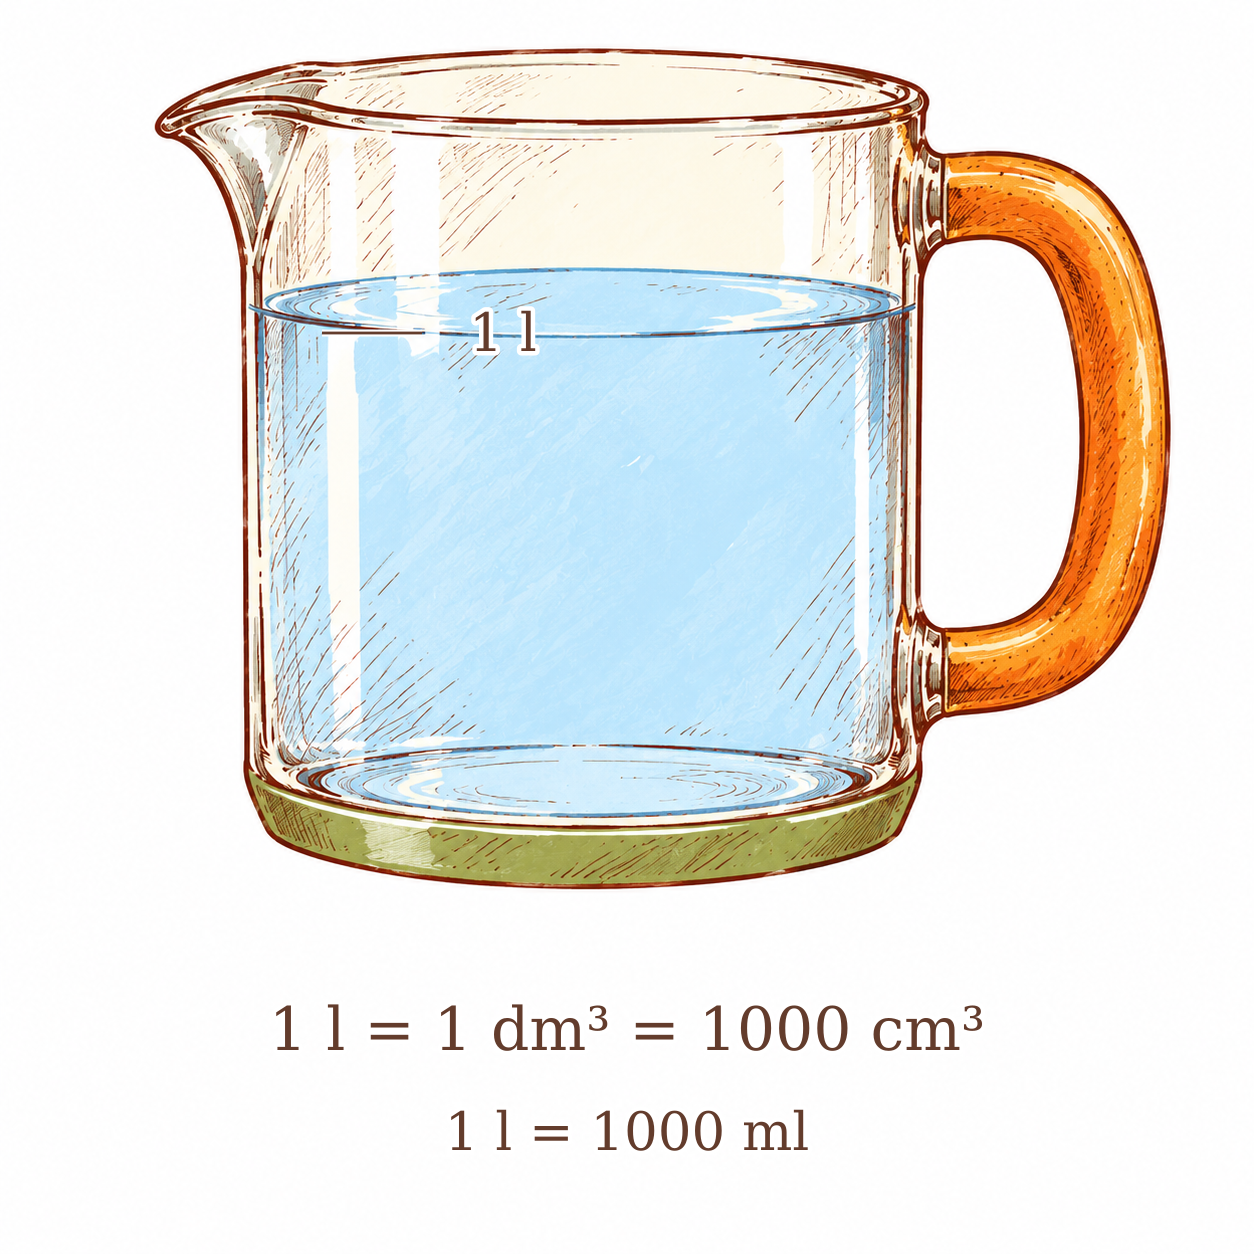
\includegraphics[width=.70\linewidth,height=55mm,keepaspectratio]{images/lota28_t7_litrar_og_rummal.png}\end{mynd}
\kafli{Tvö einingakerfi sem tengjast}
\hugtak{litri}{Lítri} og rúmdesímetri tákna sama rúmmál. \hugtak{millilitri}{Millilítri} og rúmsentímetri gera það líka.
\begin{regla}\textbf{FLÝTILEIÐ:}
\[\begin{aligned}
&1\,\text{l}=1\,\text{dm}^3\\[5pt]&1\,\text{ml}=1\,\text{cm}^3\\[5pt]&1\,\text{m}^3=1000\,\text{l}.
\end{aligned}\]
\[\begin{aligned}
&1\,\text{l}=10\,\text{dl}=100\,\text{cl}=1000\,\text{ml}.
\end{aligned}\]
Milli samliggjandi eininga \(\text{l}\to\text{dl}\to\text{cl}\to\text{ml}\) margfaldarðu með 10; í öfuga átt deilirðu með 10.\end{regla}
\begin{daemi}{Rúmeining yfir í lítra eða millilítra}
\[\begin{aligned}
&3{,}8\,\text{dm}^3=3{,}8\,\text{l}=3800\,\text{ml}\\[5pt]&275\,\text{cm}^3=275\,\text{ml}=0{,}275\,\text{l}.
\end{aligned}\]
\end{daemi}
\begin{daemi}[lotaCyan]{Lítraeining yfir í rúmeiningu}
Notum millilítra sem milliskref til að komast í \(\text{cm}^3\), en lítra til að komast í \(\text{dm}^3\):

\[\begin{aligned}
&34\,\text{cl}=340\,\text{ml}=340\,\text{cm}^3\\[5pt]&47\,\text{dl}=4{,}7\,\text{l}=4{,}7\,\text{dm}^3\\[5pt]&0{,}45\,\text{ml}=0{,}45\,\text{cm}^3.
\end{aligned}\]
\end{daemi}


\framhald{RÚMMÁL OG MASSI VATNS}
\kafli{Notaðu gefna forsendu}
\hugtak{massi}{Massi} og rúmmál eru ólíkar stærðir. Til að tengja þær þarftu að vita hve mikið tiltekið rúmmál efnis vegur. Í eftirfarandi reiknidæmum notum við nálgunina að \(1\,\text{l}\) af vatni vegi \(1\,\text{kg}\).
\begin{regla}\textbf{FLÝTILEIÐ FYRIR ÞESSI VATNSDÆMI:}
\[\begin{aligned}
&1\,\text{l}=1\,\text{dm}^3\longleftrightarrow1\,\text{kg}=1000\,\text{g}
\end{aligned}\]
\[\begin{aligned}
&1\,\text{ml}=1\,\text{cm}^3\longleftrightarrow1\,\text{g}.
\end{aligned}\]
Talnagildi rúmmáls í ml verður jafnt talnagildi massa í g \emph{með þessari forsendu}.\end{regla}
\begin{daemi}{Frá rúmmáli í grömm}
\begin{tabularx}{\linewidth}{@{}l X r@{}}
\toprule
\textbf{Vatnsmagn}&\textbf{Milliskref}&\textbf{Massi}\\\midrule
\(0{,}48\,\text{l}\)&\(480\,\text{ml}\)&\(480\,\text{g}\)\\
\(18\,\text{cm}^3\)&\(18\,\text{ml}\)&\(18\,\text{g}\)\\
\bottomrule
\end{tabularx}
\end{daemi}
\begin{daemi}[lotaCyan]{Frá massa í millilítra}
\[\begin{aligned}
&0{,}64\,\text{kg}=640\,\text{g}\longrightarrow640\,\text{ml}.
\end{aligned}\]
Prófun í hina áttina: \(640\,\text{ml}=0{,}64\,\text{l}\), sem vegur \(0{,}64\,\text{kg}\) samkvæmt forsendunni um massa vatns.

\end{daemi}
\begin{mundu}\textbf{ATH.:} Ekki nota \(1\,\text{ml}\leftrightarrow1\,\text{g}\) sjálfkrafa fyrir olíu, möl eða önnur efni. Í dæminu um möl notum við gefinn massa hvers rúmmetra. Breyta má milli rúmeininga án þess að vita hvaða efni fyllir rýmið.\end{mundu}
\clearpage
\phantomsection\label{gatlisti}
\begin{center}{\fontsize{20}{24}\selectfont\bfseries GÁTLISTI LOTU 28}\end{center}
Merktu við þegar þú getur útskýrt aðferðina og notað hana sjálfstætt. Farðu aftur í viðeigandi tíma ef þú ert óviss um eitthvert atriði.
\kafli{\hyperref[timi:lota28-01]{1. tími: Þríhyrningar og Pýþagóras}}
\gat{Ég get flokkað þríhyrning eftir bæði hornum og hliðum.}
\gat{Ég get fundið langhliðina út frá rétta horninu og reiknað óþekkta hlið.}
\gat{Ég get prófað hvort gefnar hliðarlengdir mynda rétthyrndan þríhyrning.}
\gat{Ég get teiknað hjálparmynd fyrir hornalínu, þríhyrning á þvermáli og hliðaflöt píramída.}
\gat{Ég get sett upp jöfnu þegar hliðarlengdir eru gefnar sem hlutfall.}
\kafli{\hyperref[timi:lota28-02]{2. tími: Einslögun og horn}}
\gat{Ég get nefnt reglu sem skýrir hvers vegna tvö horn eru jafn stór.}
\gat{Ég get parað saman horn og hliðar þótt myndum sé snúið eða þær speglaðar.}
\gat{Ég get sýnt einslögun þríhyrninga með tveimur hornapörum og skrifað bókstafina í réttri röð.}
\gat{Ég get fundið litla þríhyrninga inni í stærri mynd, greint hvort myndir séu einslaga, aljafnar eða hvorugt og lesið samanburðartáknin.}
\kafli{\hyperref[timi:lota28-03]{3. tími: Einslögun og hlutföll}}
\gat{Ég get fundið lengdarstuðul og notað hann á samsvarandi hliðar og hæðir.}
\gat{Ég get notað \(k^2\) til að finna flatarmál og reiknað hlutfallið sem prósentu.}
\gat{Ég get sett upp hlutfall fyrir óbeina mælingu og greint hvaða lengdir þurfa að vera þekktar.}
\gat{Ég get sameinað einslögun og Pýþagórasarreglu til að finna ummál og flatarmál hluta myndar.}
\kafli{\hyperref[timi:lota28-04]{4. tími: Mælikvarði}}
\gat{Ég get breytt lengdum í sömu einingu áður en ég stytti mælikvarða.}
\gat{Ég get greint stækkun frá minnkun og reiknað bæði myndlengd og raunlengd.}
\gat{Ég get fundið mælikvarða með mælingu og útskýrt áhrif prentstærðar.}
\gat{Ég get breytt flatarmáli á korti í raunverulegt flatarmál með réttum einingum.}
\newpage
\kafli{\hyperref[timi:lota28-05]{5. tími: Mælikvarðar og vinnuteikningar}}
\gat{Ég get talið reitabil, reiknað lengdir sniðs og tekið tillit til brots í efni.}
\gat{Ég get sýnt hvernig snið rúmast á gefinni efnisbreidd og skráð forsendur um saumför og afskurð.}
\gat{Ég get gert efnislista með fjölda, stykkjalengd og heildarlengd fyrir hverja efnisgerð.}
\gat{Ég get teiknað grunnmynd, mynd framan frá og mynd frá hlið í sama kvarða og merkt raunmálin.}
\gat{Ég get reiknað flatarmál gólfs og áætlað hversu stóran hluta þess búnaður þekur.}
\gat{Ég get yfirfært mál á þrjár stefnur þrívíddarpunktanets.}
\kafli{\hyperref[timi:lota28-06]{6. tími: Flatarmál, ummál og rúmmál}}
\gat{Ég get valið rétta formúlu og einingu fyrir ummál, flatarmál og rúmmál.}
\gat{Ég get fundið rétta hæð þríhyrnings, einnig þegar hún liggur utan hans eða þarf að reikna hana.}
\gat{Ég get borið saman hring og ferning með reikningi og greint radíus frá þvermáli.}
\gat{Ég get notað \(R=Gh\), fundið möguleg kassamál og reiknað massa þegar massi á rúmmetra er gefinn.}
\gat{Ég get fundið rúmmál samsetts forms með samlagningu eða frádrætti án tvítalningar.}
\kafli{\hyperref[timi:lota28-07]{7. tími: Rúmmál og einingabreytingar}}
\gat{Ég get útskýrt hvers vegna stuðullinn er 1000 við hvert skref í einingastiganum.}
\gat{Ég get breytt í báðar áttir milli \(\text{m}^3\), \(\text{dm}^3\), \(\text{cm}^3\) og \(\text{mm}^3\).}
\gat{Ég get breytt milli l, dl, cl og ml og tengt þær einingar við rúmeiningar.}
\gat{Ég get fundið massa eða rúmmál vatns með gefinni forsendu og prófað svarið í hina áttina.}

\clearpage
\phantomsection\label{hugtok}
\begin{center}{\fontsize{20}{24}\selectfont\bfseries HUGTÖK LOTUNNAR}\end{center}
Smelltu á tilvísun við hugtak til að fara aftur í umfjöllun þess.
\kafli{Þríhyrningar og lengdir}
\gloss{hornasumma}{Hornasumma}{Summa allra innri horna marghyrnings. Í þríhyrningi er hún \(180^\circ\).}{1}
\gloss{hvasshyrndur}{Hvasshyrndur þríhyrningur}{Þríhyrningur þar sem öll horn eru minni en \(90^\circ\).}{1}
\gloss{retthyrndur}{Rétthyrndur þríhyrningur}{Þríhyrningur með eitt rétt horn, \(90^\circ\).}{1}
\gloss{gleidhyrndur}{Gleiðhyrndur þríhyrningur}{Þríhyrningur með eitt horn stærra en \(90^\circ\).}{1}
\gloss{jafnhlida}{Jafnhliða þríhyrningur}{Þríhyrningur með þrjár jafnlangar hliðar. Öll horn hans eru \(60^\circ\).}{1}
\gloss{jafnarma}{Jafnarma þríhyrningur}{Þríhyrningur með að minnsta kosti tvær jafnlangar hliðar. Hornin gegnt þeim eru jafn stór.}{1}
\gloss{langhlid}{Langhlið}{Hliðin gegnt rétta horninu í rétthyrndum þríhyrningi. Hún er lengsta hlið hans.}{1}
\gloss{skammhlid}{Skammhlið}{Önnur tveggja hliða sem mynda rétta hornið í rétthyrndum þríhyrningi.}{1}
\gloss{pythagoras}{Pýþagórasarregla}{Í rétthyrndum þríhyrningi er \(a^2+b^2=c^2\), þar sem \(c\) er lengd langhliðarinnar og \(a,b\) lengdir skammhliðanna.}{1}
\gloss{hornalina}{Hornalína}{Strik sem tengir tvo hornpunkta marghyrnings sem liggja ekki við sömu hlið. Hornalína rétthyrnings myndar rétthyrndan þríhyrning með tveimur hliðum hans.}{1}
\gloss{haed}{Hæð}{Hornrétt fjarlægð. Í þríhyrningi er hæðin fjarlægðin frá hornpunkti að línunni sem mótlæg hlið liggur á.}{1}
\gloss{thvermal}{Þvermál}{Strik milli tveggja punkta á hringferli sem liggur gegnum miðju hrings, eða lengd þess. Lengdin er \(\text{þ}=2r\).}{1}

\newpage
\kafli{Horn, einslögun og kvarði}
\gloss{grannhorn}{Grannhorn}{Tvö samliggjandi horn með sameiginlegan arm, þar sem hinir armarnir mynda beina línu. Summa þeirra er \(180^\circ\).}{2}
\gloss{topphorn}{Topphorn}{Gagnstæð horn við skurðpunkt tveggja lína. Armar annars hornsins eru framhald af örmum hins. Topphorn eru jafn stór.}{2}
\gloss{samsida}{Samsíða línur}{Línur í sama fleti sem skerast ekki. Táknað \(l\parallel m\).}{2}
\gloss{einslaeg}{Einslæg horn}{Horn í samsvarandi stöðu þar sem lína sker tvær aðrar línur. Þegar þær tvær eru samsíða eru einslægu hornin jafn stór.}{2}
\gloss{einslaga}{Einslaga myndir}{Myndir með sömu lögun: samsvarandi horn eru jafn stór og hlutfall samsvarandi lengda er fast. Táknið er \(\sim\). Myndirnar geta verið jafnstórar eða misstórar.}{2}
\gloss{aljafn}{Aljafnar myndir}{Myndir með sömu lögun og stærð. Samsvarandi hliðar eru jafn langar og horn jafn stór. Táknið er \(\cong\).}{2}
\gloss{jafnadarmerki}{Jafnaðarmerki}{Táknið \(=\) segir að gildið sé hið sama báðum megin. \(AB=DE\) merkir að lengdir strikanna séu jafnar; \(\angle ABC=\angle DEF\) að hornastærðirnar séu jafnar.}{2}
\gloss{nalgunarmerki}{Nálgunarmerki}{Táknið \(\approx\) merkir um það bil jafnt og. Til dæmis er \(\sqrt{2}\approx1{,}41\), þar sem svarið er námundað að tveimur aukastöfum.}{2}
\gloss{hornrett}{Hornréttar línur}{Línur sem skerast undir réttu horni, \(90^\circ\). \(l\perp m\) er lesið: l er hornrétt á m.}{2}
\gloss{samsvorun}{Samsvörun}{Pörun hornpunkta eða hliða sem hafa sömu stöðu þegar myndir eru bornar saman. Í \(\triangle ABC\sim\triangle PQR\) samsvarar A punktinum P, B punktinum Q og C punktinum R. Örin \(\leftrightarrow\) sýnir þessa pörun.}{2}
\gloss{staekkunarstudull}{Stækkunarstuðull}{Hlutfallið \(k=\frac{\text{ný lengd}}{\text{upphafleg lengd}}\) milli samsvarandi lengda í einslaga myndum. \(k>1\) gefur stækkun, \(0<k<1\) minnkun og \(k=1\) óbreytta stærð.}{3}
\gloss{maelikvardi}{Mælikvarði}{Hlutfall myndlengdar og raunlengdar í sömu einingu. Í \(1:200\) táknar \(1\cm\) á mynd \(200\cm\) í raun.}{4}
\kafli{Vinnuteikningar}
\gloss{vinnuteikning}{Vinnuteikning}{Teikning sem sýnir stærð og gerð hlutar með málum, einingum og myndum frá viðeigandi sjónarhornum. Mælikvarði skal koma fram þegar teiknað er í kvarða.}{5}
\gloss{efnislisti}{Efnislisti}{Skrá um efnisgerðir, fjölda stykkja, mál þeirra og heildarmagn efnis sem þarf í verkið.}{5}
\gloss{grunnmynd}{Grunnmynd}{Sýn ofan frá sem sýnir lengd, breidd og innbyrðis staðsetningu hluta.}{5}
\gloss{framsyn}{Mynd framan frá}{Sýn beint framan á hlut sem sýnir breidd hans og hæð.}{5}
\gloss{hlidarsyn}{Mynd frá hlið}{Sýn beint á hlið hlutar sem sýnir dýpt eða lengd hans og hæð.}{5}
\gloss{thrividd}{Þrívíddarteikning}{Mynd sem sýnir þrjár víddir hlutar, lengd, breidd og hæð. Skáhallar stefnur á blaði sýna dýpt.}{5}

\newpage
\kafli{Flötur, rými og einingar}
\gloss{ummal}{Ummál}{Lengd jaðars flatar. Mælt í lengdareiningum, til dæmis cm eða m.}{6}
\gloss{flatarmal}{Flatarmál}{Stærð flatar. Mælt í ferningseiningum, til dæmis cm\(^2\) eða m\(^2\).}{6}
\gloss{rummal}{Rúmmál}{Stærð rýmis sem hlutur fyllir eða ílát getur rúmað. Mælt til dæmis í cm\(^3\), dm\(^3\), m\(^3\) eða lítrum.}{6}
\gloss{radius}{Radíus}{Fjarlægð frá miðju hrings að hringferli, táknuð \(r\). Þvermálið er \(2r\).}{6}
\gloss{rettstrendingur}{Réttstrendingur}{Strendingur með tvo samsíða, eins grunnfleti þar sem hliðarbrúnir eru hornréttar á grunnfletina. Rúmmálið fæst með því að margfalda flatarmál grunnflatarins með hæðinni: \(R=Gh\).}{6}
\gloss{litri}{Lítri}{Rúmmálseining: \(1\,\text{l}=1\,\text{dm}^3=1000\,\text{ml}\). Desílítri er \(0{,}1\,\text{l}\) og sentílítri \(0{,}01\,\text{l}\).}{7}
\gloss{millilitri}{Millilítri}{Einn þúsundasti úr lítra: \(1\,\text{ml}=0{,}001\,\text{l}=1\,\text{cm}^3\).}{7}
\gloss{massi}{Massi}{Stærð sem meðal annars er mæld í grömmum, kílógrömmum eða tonnum. Sama rúmmál ólíkra efna getur haft ólíkan massa. \(1\,\text{kg}=1000\,\text{g}\) og \(1\) tonn \(=1000\,\text{kg}\).}{7}
\end{document}
